\documentclass[compress]{beamer}
\usepackage{ifthen,verbatim}

\newcommand{\isnote}{}
\xdefinecolor{lightyellow}{rgb}{1.,1.,0.25}
\xdefinecolor{darkblue}{rgb}{0.1,0.1,0.7}

%% Uncomment this to get annotations
%% \def\notes{\addtocounter{page}{-1}
%%            \renewcommand{\isnote}{*}
%% 	   \beamertemplateshadingbackground{lightyellow}{white}
%%            \begin{frame}
%%            \frametitle{Notes for the previous page (page \insertpagenumber)}
%%            \itemize}
%% \def\endnotes{\enditemize
%% 	      \end{frame}
%%               \beamertemplateshadingbackground{white}{white}
%%               \renewcommand{\isnote}{}}

%% Uncomment this to not get annotations
\def\notes{\comment}
\def\endnotes{\endcomment}

\setbeamertemplate{navigation symbols}{}
\setbeamertemplate{headline}{\mbox{ } \hfill
\begin{minipage}{5.5 cm}
\vspace{-0.75 cm} \small
\end{minipage} \hfill
\begin{minipage}{4.5 cm}
\vspace{-0.75 cm} \small
\begin{flushright}
\ifthenelse{\equal{\insertpagenumber}{1}}{}{Jim Pivarski \hspace{0.2 cm} \insertpagenumber\isnote/\pageref{numpages}}
\end{flushright}
\end{minipage}\mbox{\hspace{0.2 cm}}\includegraphics[height=1 cm]{../cmslogo} \hspace{0.1 cm} \includegraphics[height=1 cm]{../tamulogo} \hspace{0.01 cm} \vspace{-1.05 cm}}

\begin{document}
\begin{frame}
\vfill
\begin{center}
\textcolor{darkblue}{\Large Status of Track-based Geometry in the Endcap}

\vfill
\begin{columns}
\column{0.3\linewidth}
\begin{center}
\large
\textcolor{darkblue}{Jim Pivarski}

\vspace{0.2 cm}
Alexei Safonov
\end{center}

\column{0.3\linewidth}
\begin{center}
\large
K\'aroly Banicz
\end{center}
\end{columns}

\begin{columns}
\column{0.3\linewidth}
\begin{center}
\scriptsize
{\it Texas A\&M University}
\end{center}
\column{0.3\linewidth}
\begin{center}
\scriptsize
{\it US-CMS}
\end{center}
\end{columns}

\vfill
12 December, 2008

\end{center}
\end{frame}

%% \begin{notes}
%% \item This is the annotated version of my talk.
%% \item If you want the version that I am presenting, download the one
%% labeled ``slides'' on Indico (or just ignore these yellow pages).
%% \item The annotated version is provided for extra detail and a written
%% record of comments that I intend to make orally.
%% \item Yellow notes refer to the content on the {\it previous} page.
%% \item All other slides are identical for the two versions.
%% \end{notes}

\small

\begin{frame}
\frametitle{Outline}
\begin{itemize}\setlength{\itemsep}{0.75 cm}
\item CSC Overlaps results in more detail
\item Plan to align endcap disks/rings with standAloneMuons, with cross-checks
\item Proposed procedure for combining photogrammetry, hardware, and
  track-based results in the endcap
\end{itemize}
%% \hspace{-0.83 cm} \textcolor{darkblue}{\Large Outline2}

\vfill
\mbox{ }
\end{frame}

\begin{frame}
\frametitle{Motivation for CSC Overlaps}
\begin{itemize}
\item Baseline alignment procedure shown to require 10--100~pb$^{-1}$ for a few hundred micron precision
\item Quicker alternative:
\begin{enumerate}\setlength{\itemsep}{0.1 cm}
\item relative alignment of chambers in each ring (CSC Overlaps)
\item align whole ring with a small number of quality tracks
\end{enumerate}
\item Particularly good for layer alignment
\end{itemize}

\begin{columns}
\column{0.5\linewidth}
Overlaps chamber alignment:
\begin{enumerate}\setlength{\itemsep}{0 cm}
\item select tracks that pass through overlap of chambers in a ring
\item require consistency in pair of segments: slope and intercept
\item solve system
\end{enumerate}

\column{0.2\linewidth}
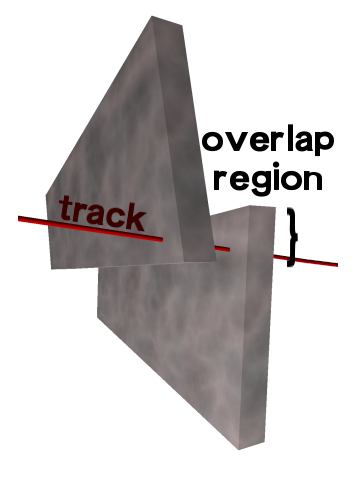
\includegraphics[width=\linewidth]{overlaps.png}

\column{0.3\linewidth}
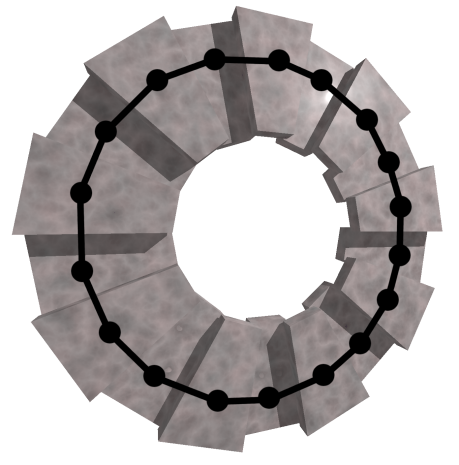
\includegraphics[width=\linewidth]{one_station.png}
\end{columns}

\vfill
System is over-constrained: must be consistent with a circle (``closure'')
\end{frame}

\begin{frame}
\frametitle{Three-step procedure}

Interdependencies between alignment parameters are unidirectional

\begin{enumerate}\setcounter{enumi}{-1}
\item Fit segment of track in each chamber to $\phi(z) = a + bz$
\item Align $\varphi_y$ angles (rotation around vertical axis) \hfill $\Delta b \to 0$
\item Align $r\phi$ positions (rotation around beamline) \hfill $\Delta a \to 0$
\item Align $\varphi_z$ angles (rotation in the detector plane) \hfill $d(\Delta a)/dy \to 0$
\end{enumerate}

\begin{columns}
\column{0.35\linewidth}
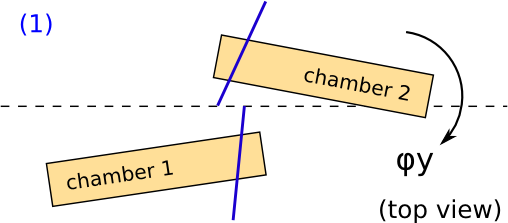
\includegraphics[width=\linewidth]{topview_1.png}
\column{0.01\linewidth}
\hfill $\to$ \hfill
\column{0.35\linewidth}
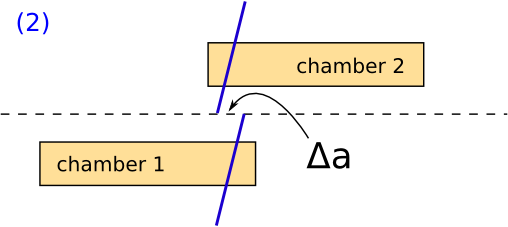
\includegraphics[width=\linewidth]{topview_2.png}
\column{0.01\linewidth}
\hfill $\to$ \hfill
\column{0.25\linewidth}
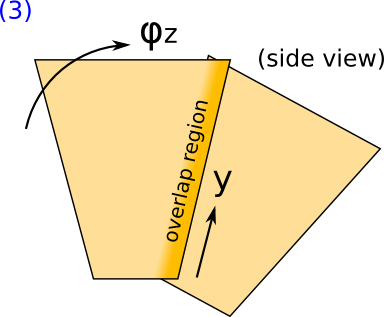
\includegraphics[width=\linewidth]{sideview.png}
\end{columns}

\vfill
\begin{itemize}
\item Parameters decouple when aligned in this order (for example,
  $\varphi_y$ depends only on $\Delta b$, but $r\phi$ depends on
  $\Delta a$ and $\Delta b$)
\item These are all of the rigid-body parameters accessible to \mbox{overlaps tracks\hspace{-1 cm}}
\end{itemize}
\end{frame}

\begin{frame}
\frametitle{Demonstration in Monte Carlo}

\begin{itemize}
\item Randomly misalign chambers and apply procedure using beam-halo Monte Carlo
\begin{itemize}
\item statistics are roughly the same as September beam-halo
\item some chambers have more tracks, others less because $\phi$ distribution not perfectly modeled
\end{itemize}
\item Plot aligned position minus true position in simulation (resolution)
\item Unaligned is grey, aligned is yellow; one histogram entry \mbox{per chamber\hspace{-1 cm}}
\begin{itemize}
\item $\delta \varphi_y \sim 1$~mrad, \hspace{0.2 cm} $\delta r\phi \sim 230$~$\mu$m, \hspace{0.2 cm} $\delta \varphi_z \sim 0.25$~mrad
\end{itemize}
\end{itemize}

\vfill
\begin{columns}
\column{0.33\linewidth}
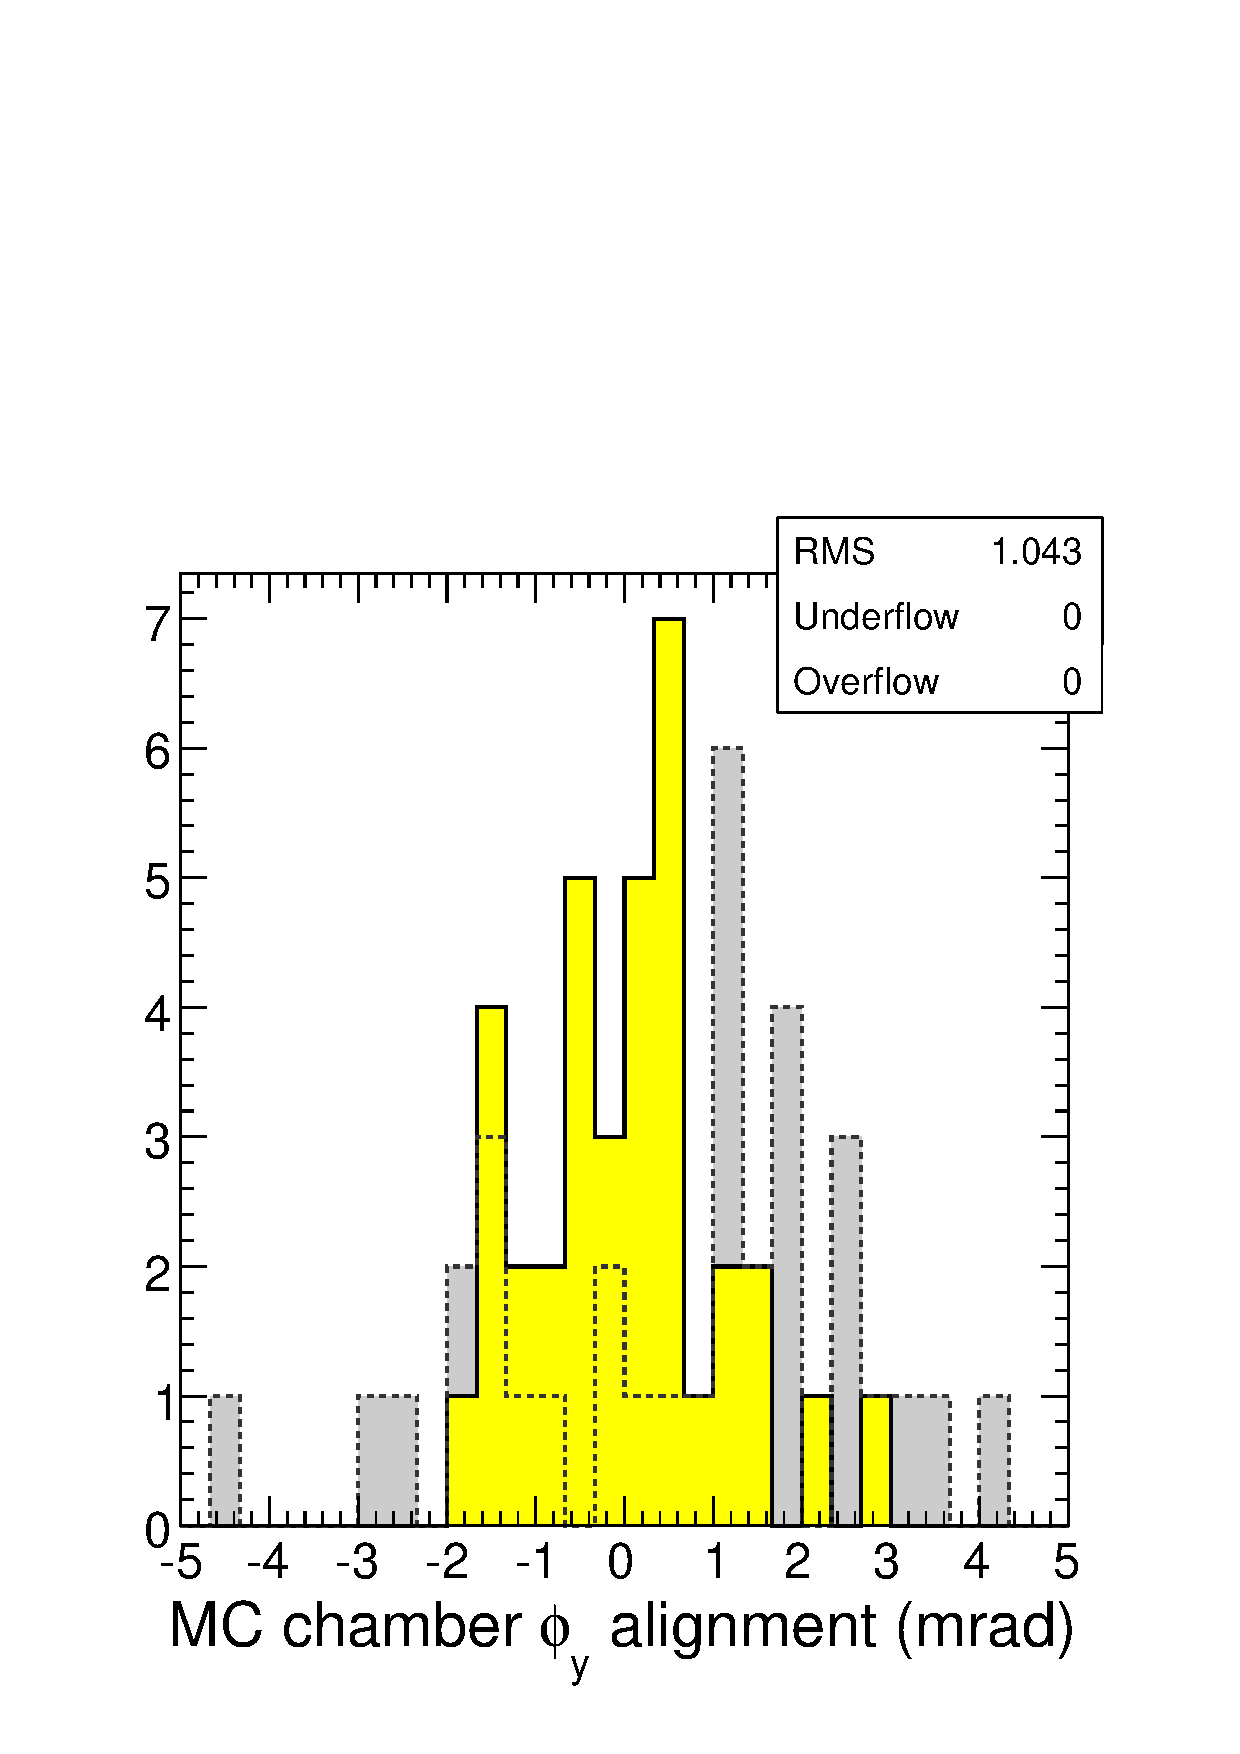
\includegraphics[width=\linewidth]{mcchamber_phiy.pdf}
\column{0.33\linewidth}
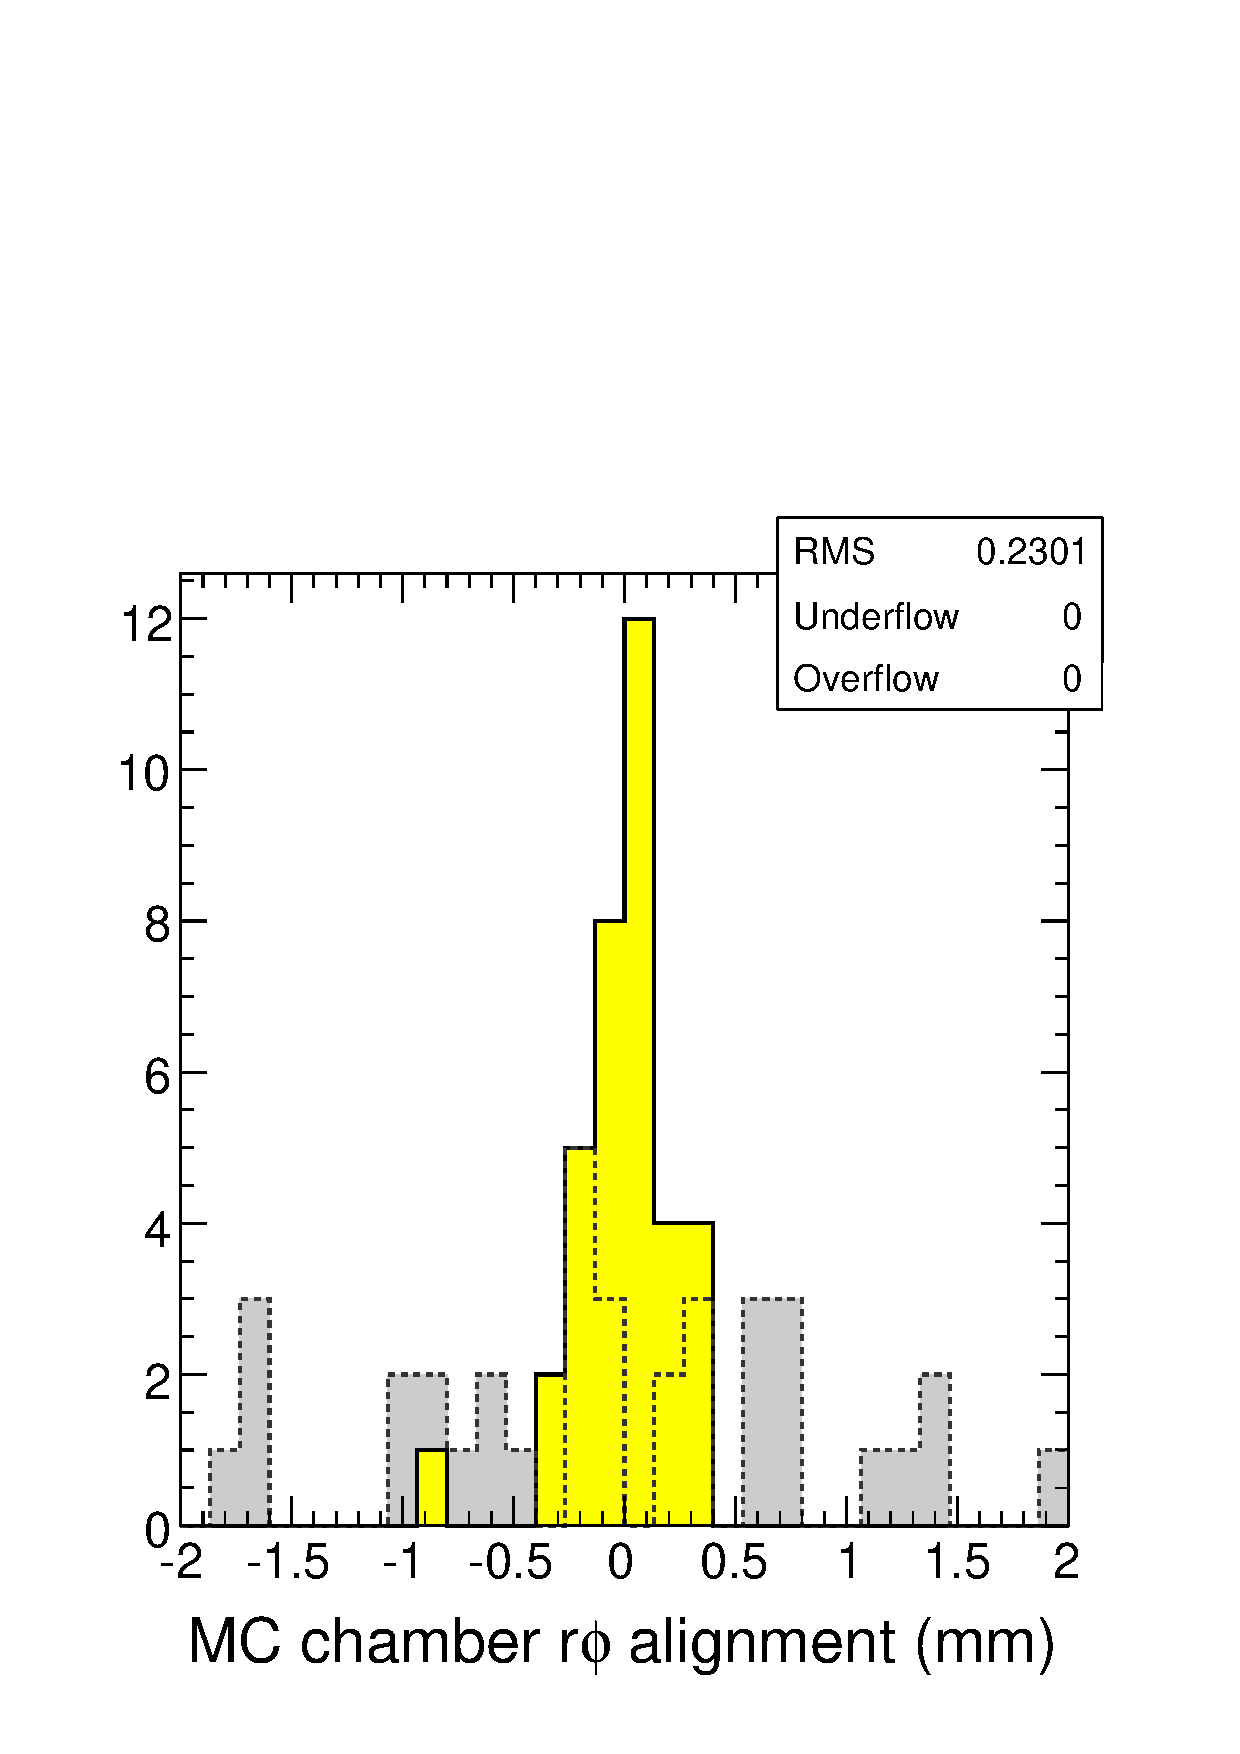
\includegraphics[width=\linewidth]{mcchamber_rphi.pdf}
\column{0.33\linewidth}
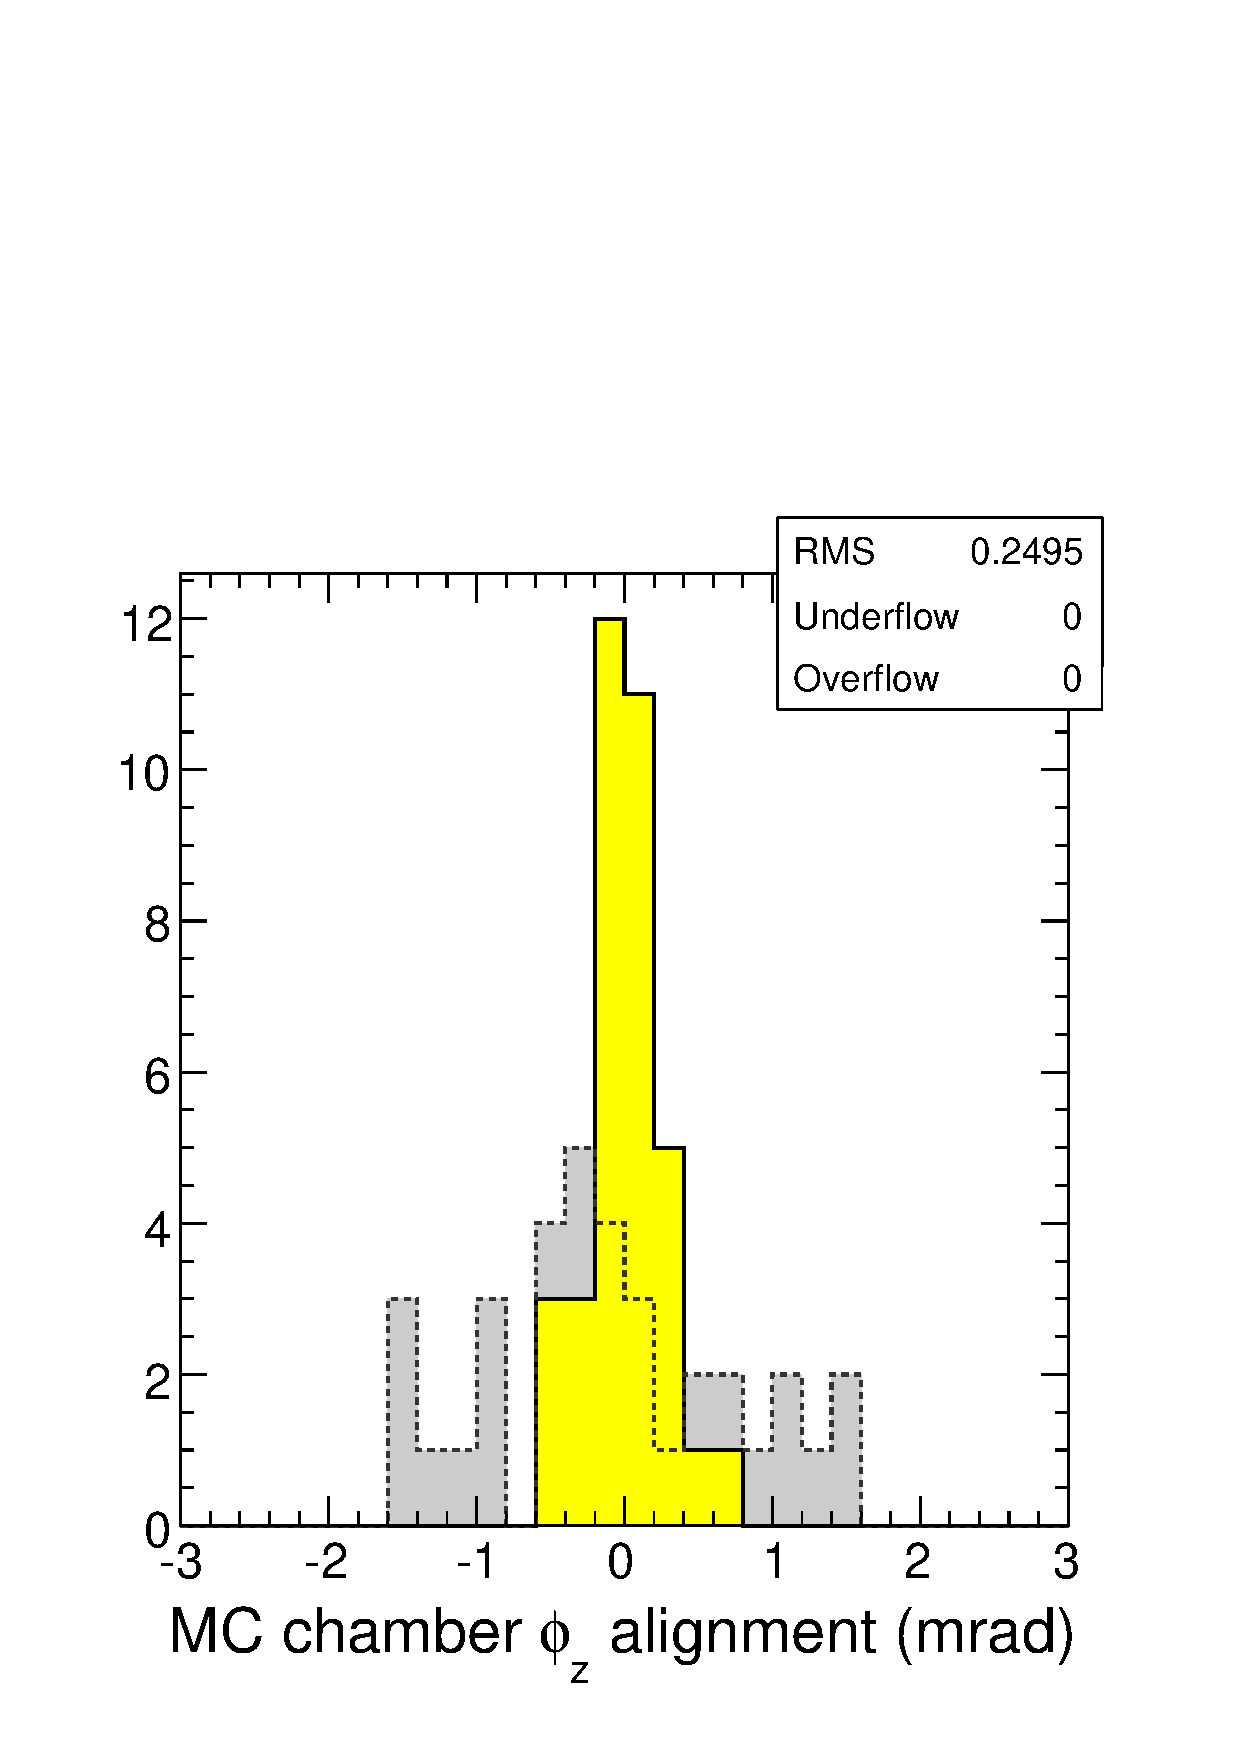
\includegraphics[width=\linewidth]{mcchamber_phiz.pdf}
\end{columns}
\end{frame}

\begin{frame}
\frametitle{Alignment in real data}

\vfill
\begin{columns}
\column{0.5\linewidth}
\begin{itemize}
\item Aligned \only<1>{\textcolor{darkblue}{ME$-$2/1}}\only<2>{ME$-$2/1} and \only<1>{ME$-$3/1}\only<2>{\textcolor{darkblue}{ME$-$3/1}} using beam-halo data
\item Compared with \mbox{photogrammetry\hspace{-1 cm}}
\begin{itemize}
\item only track-based alignment sensitive to $\varphi_y$

(only two alignment pins)
\end{itemize}
\item Plot corrections relative to ideal geometry for \mbox{each chamber\hspace{-1 cm}}
\begin{itemize}
\item track-based: \mbox{solid histogram\hspace{-1 cm}}
\item photogrammetry: \mbox{blue points\hspace{-1 cm}}
\end{itemize}
\item Physical misalignments are $\sim$2~mrad in $\varphi_y$, 1~mm in $r\phi$, and 1~mrad in $\varphi_z$
\item Corrections from independent methods follow each \mbox{other closely\hspace{-1 cm}}
\end{itemize}

\column{0.49\linewidth}
\only<1>{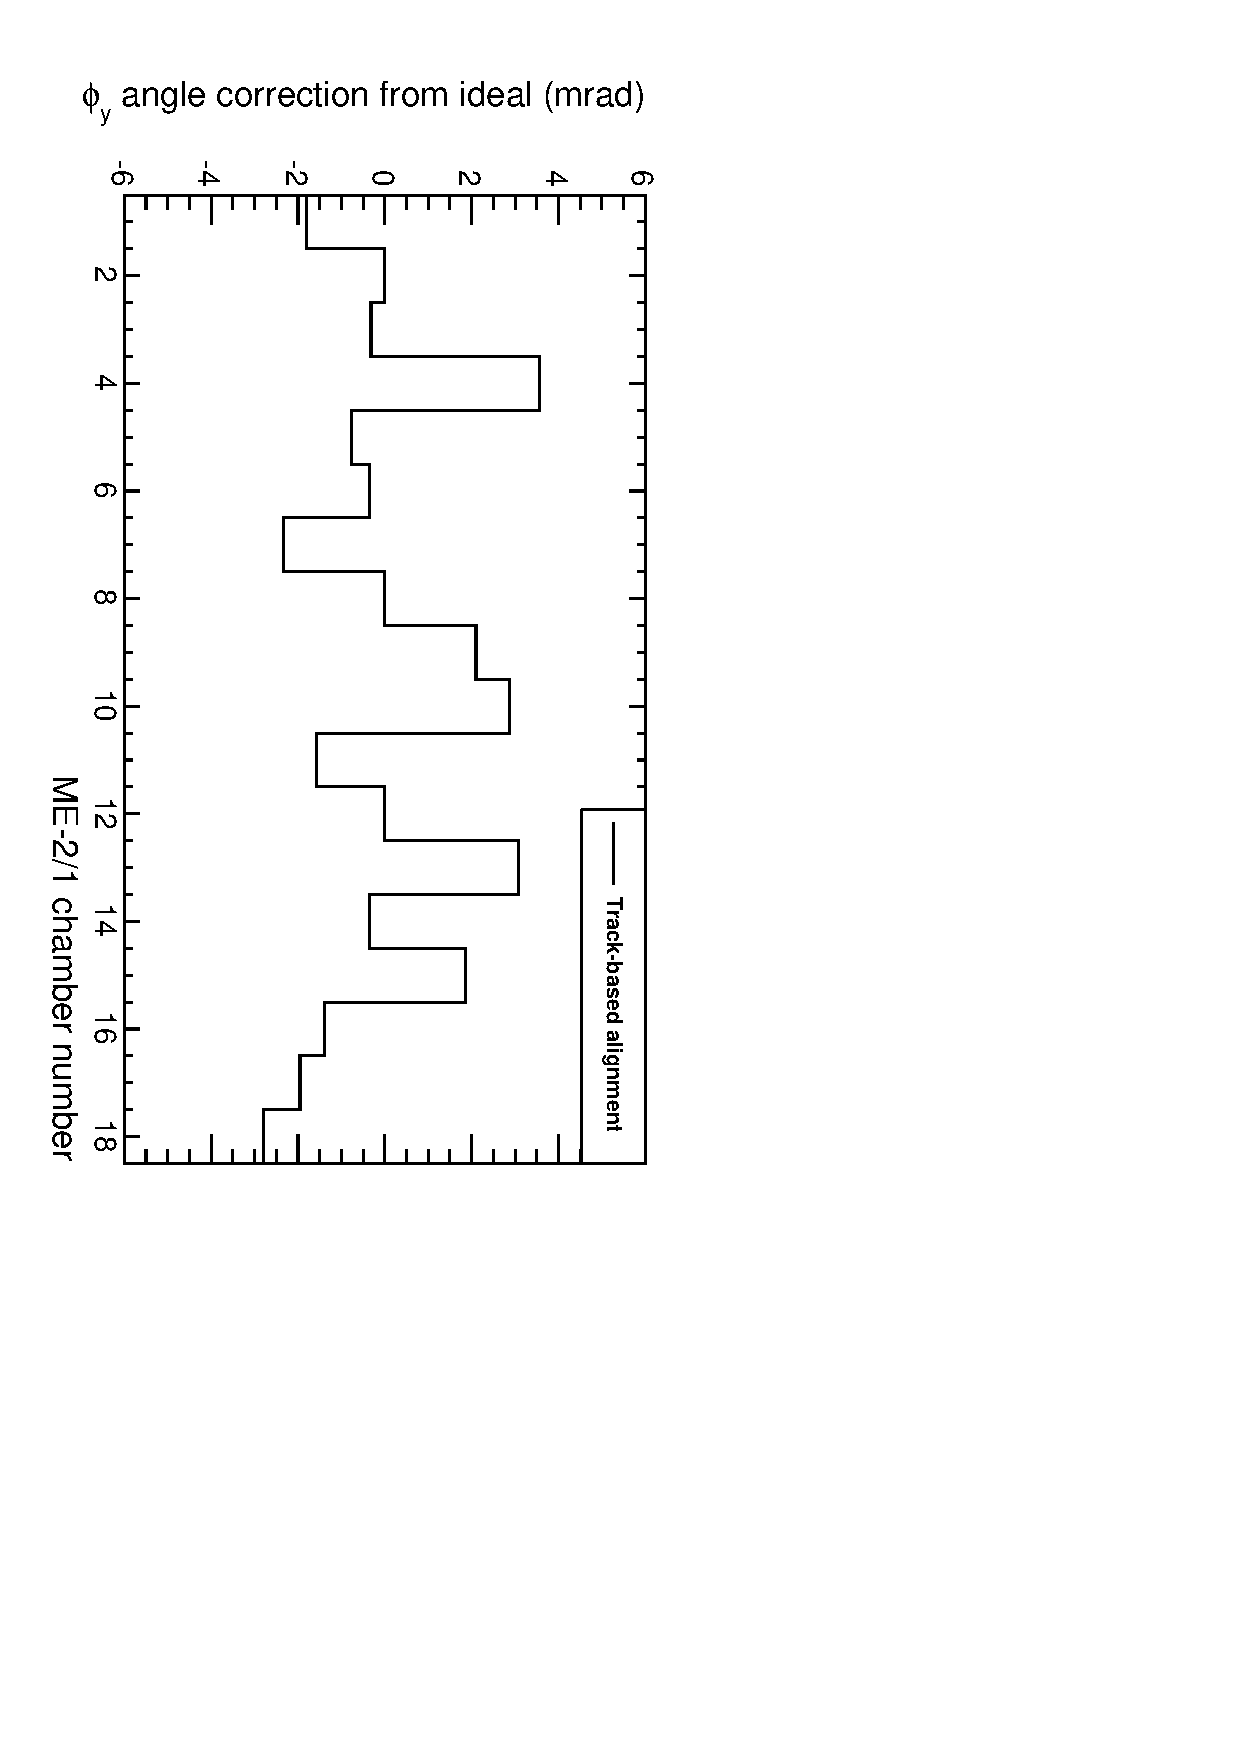
\includegraphics[height=0.95\linewidth, angle=90]{compare_m21_phiy.pdf}}\only<2>{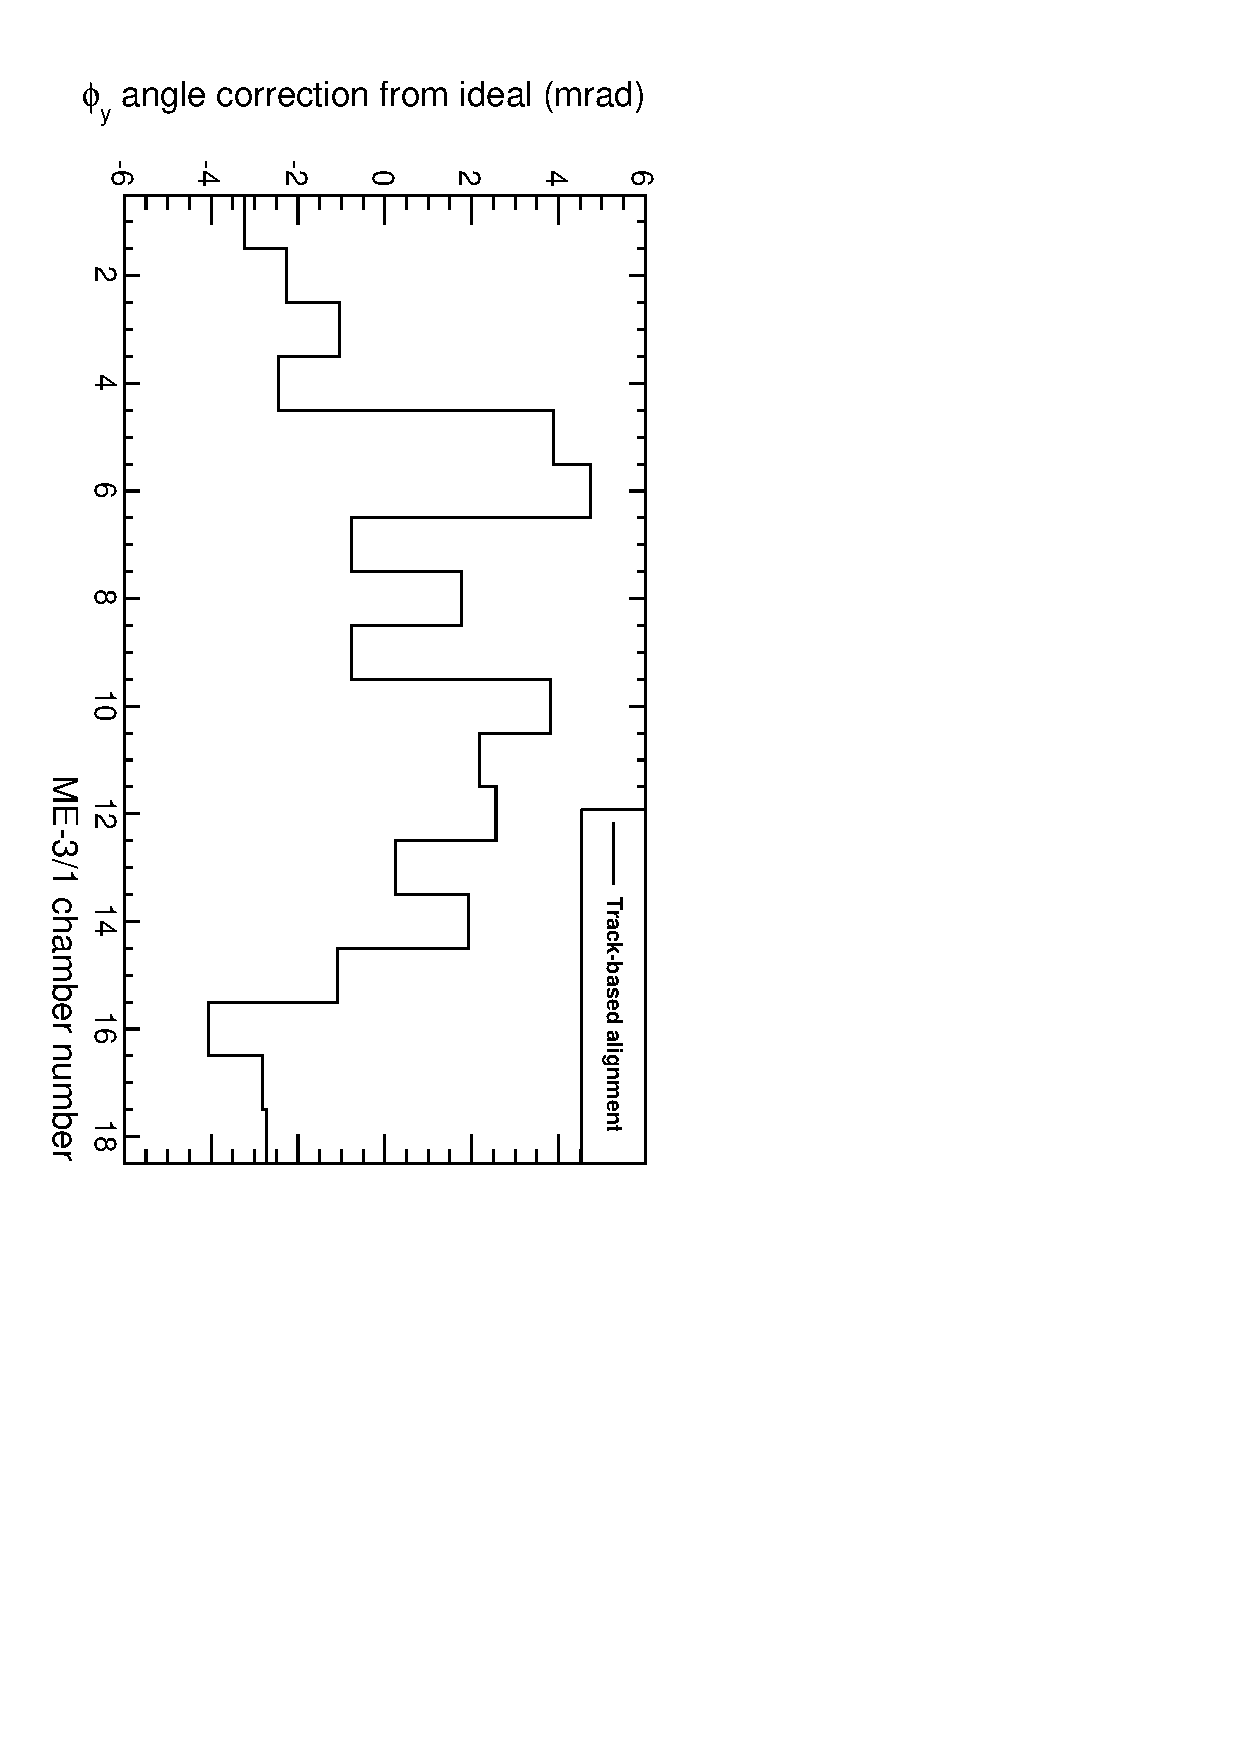
\includegraphics[height=0.95\linewidth, angle=90]{compare_m31_phiy.pdf}} \\
\only<1>{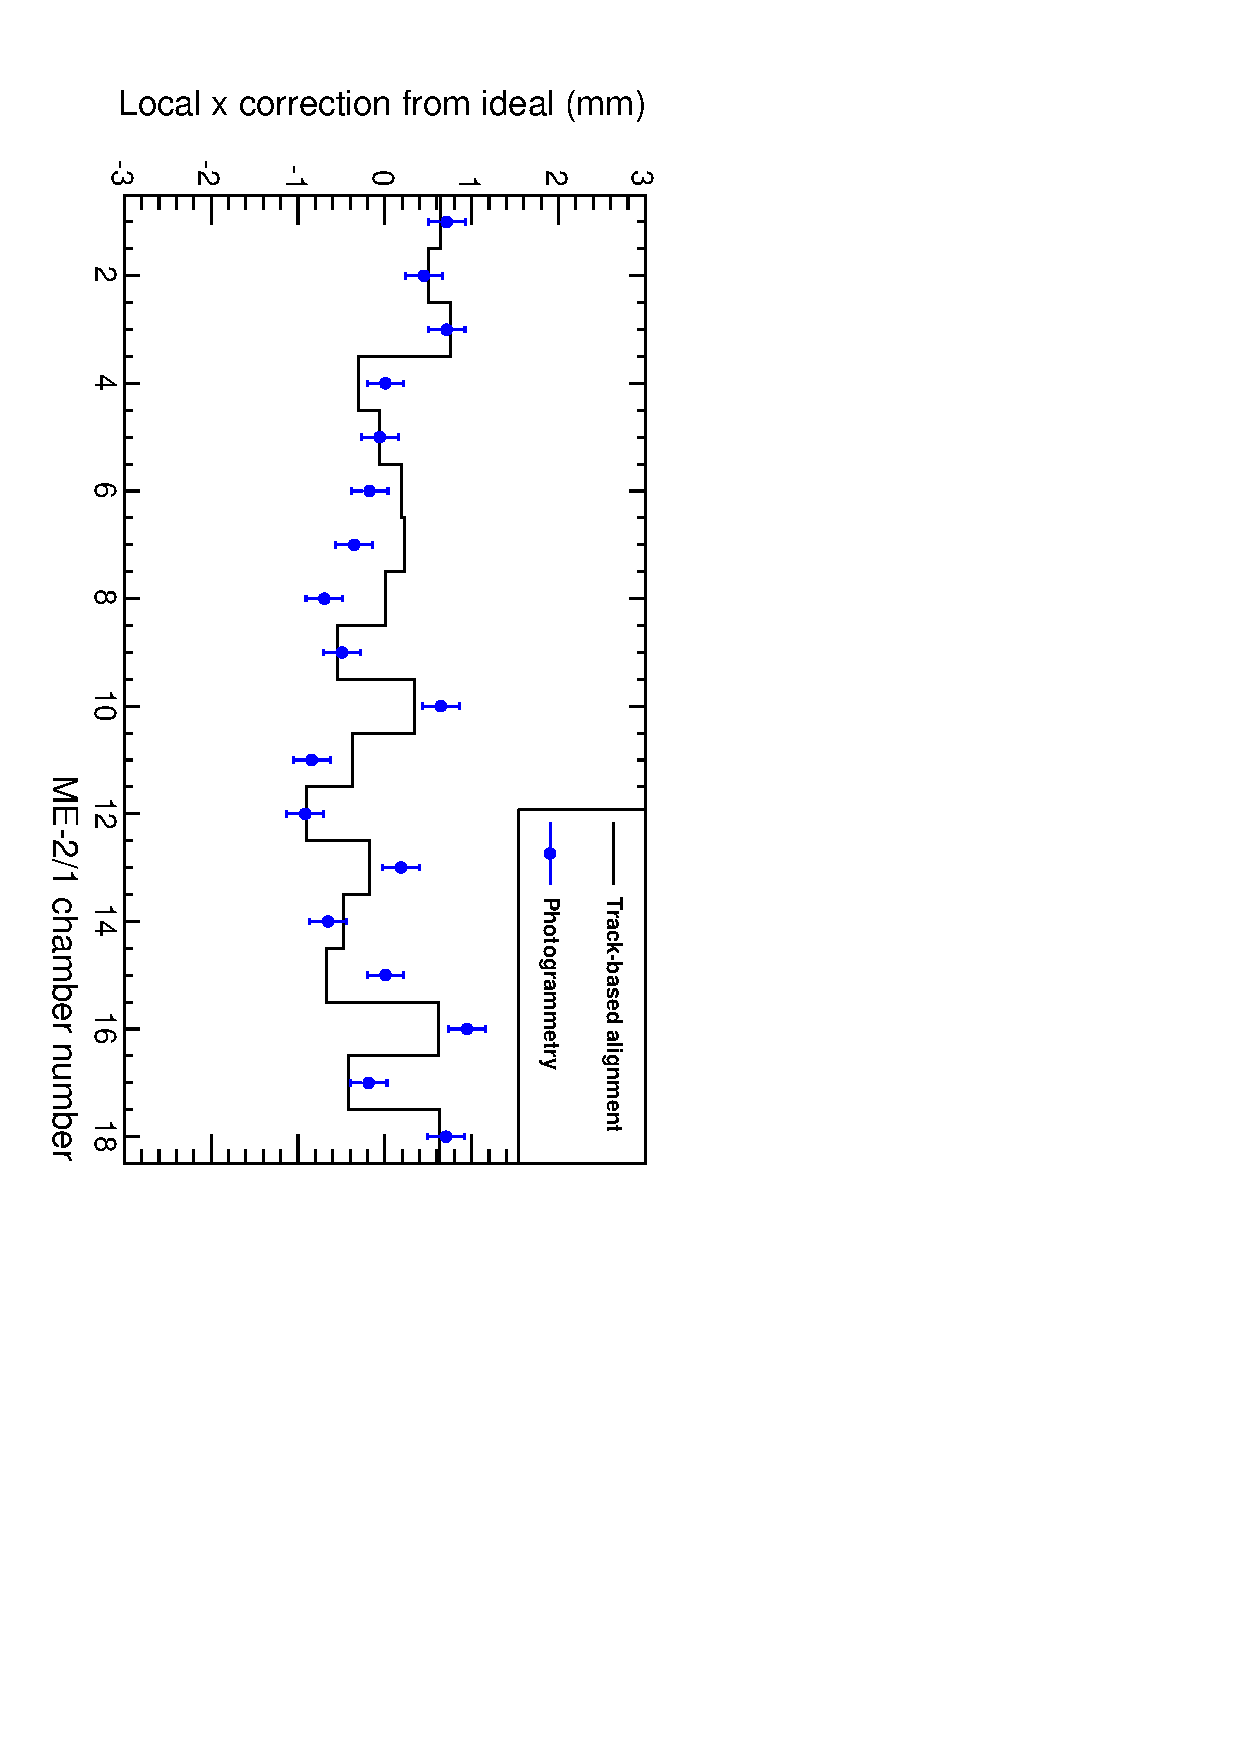
\includegraphics[height=0.95\linewidth, angle=90]{compare_m21_x.pdf}}\only<2>{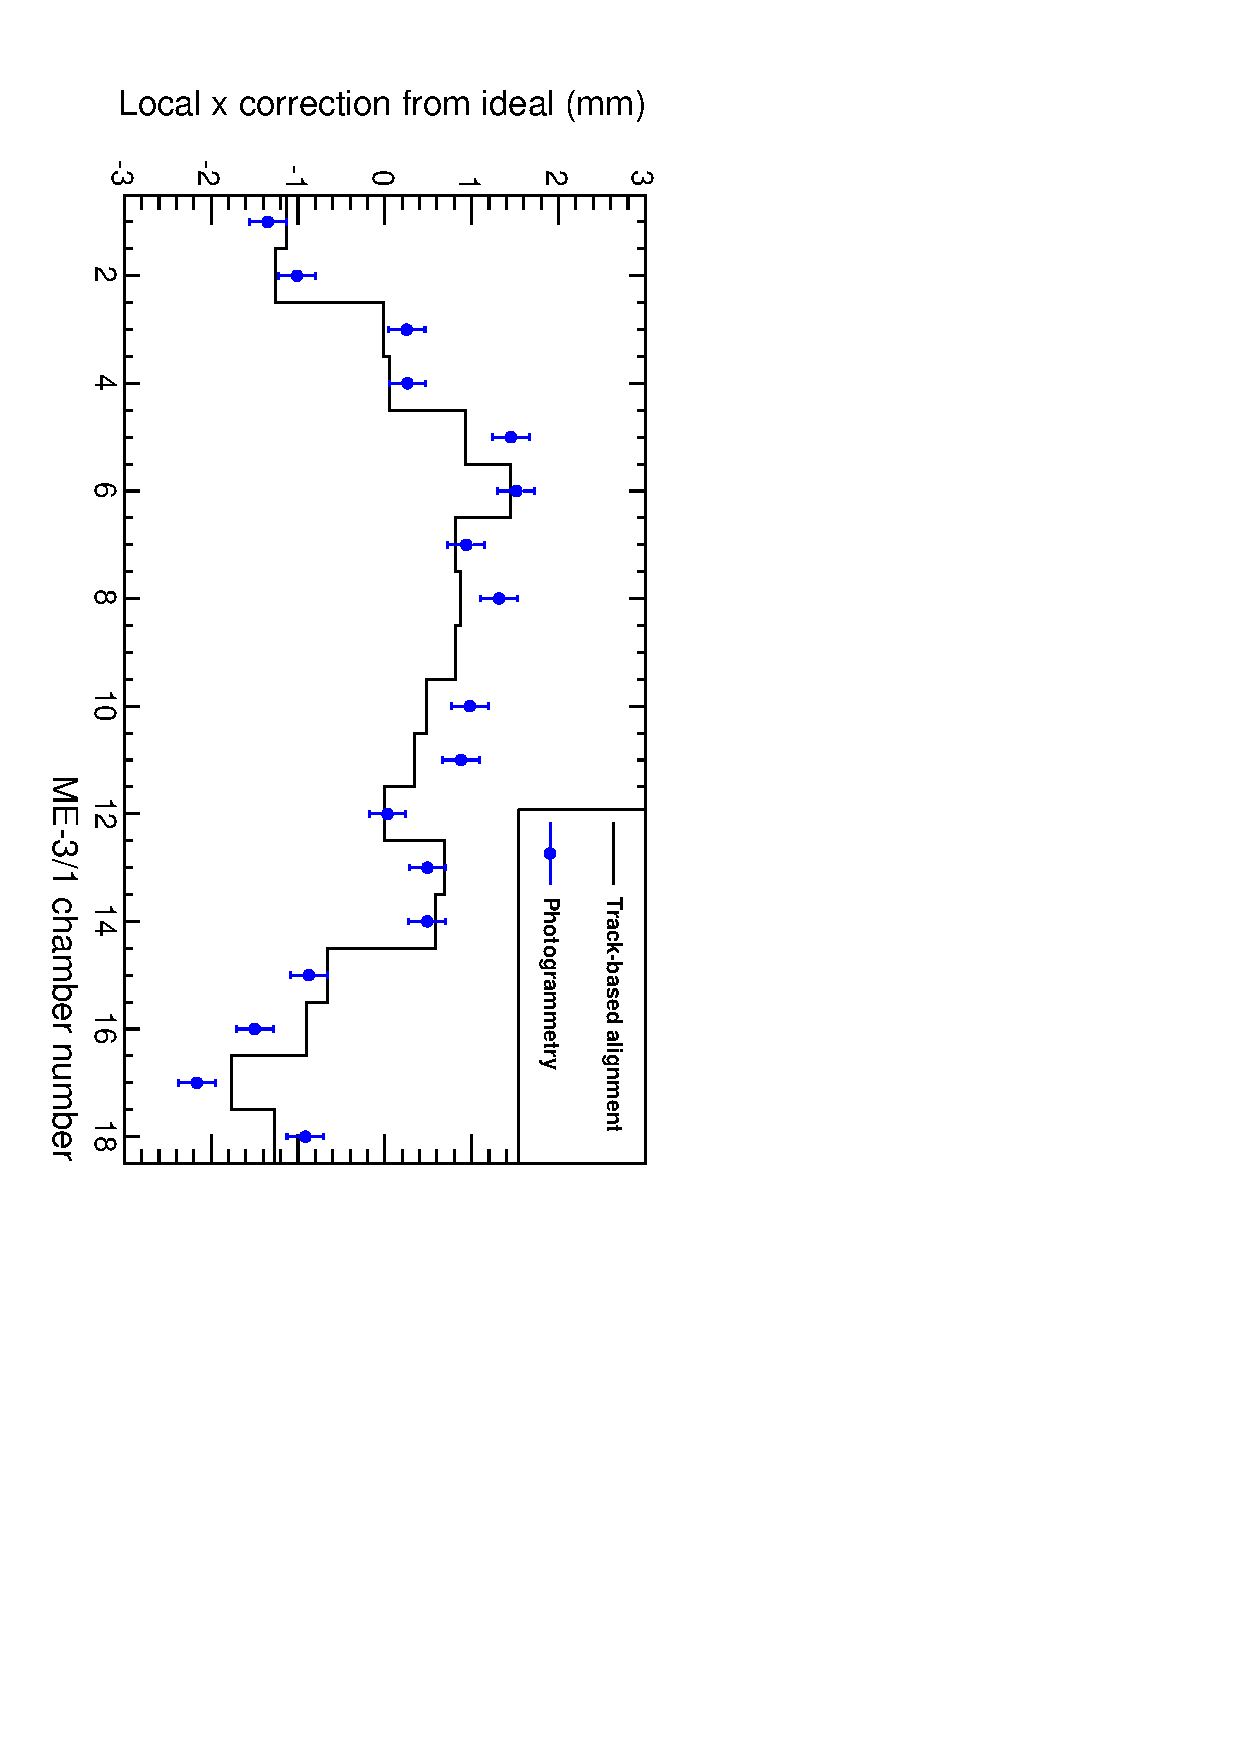
\includegraphics[height=0.95\linewidth, angle=90]{compare_m31_x.pdf}} \\
\only<1>{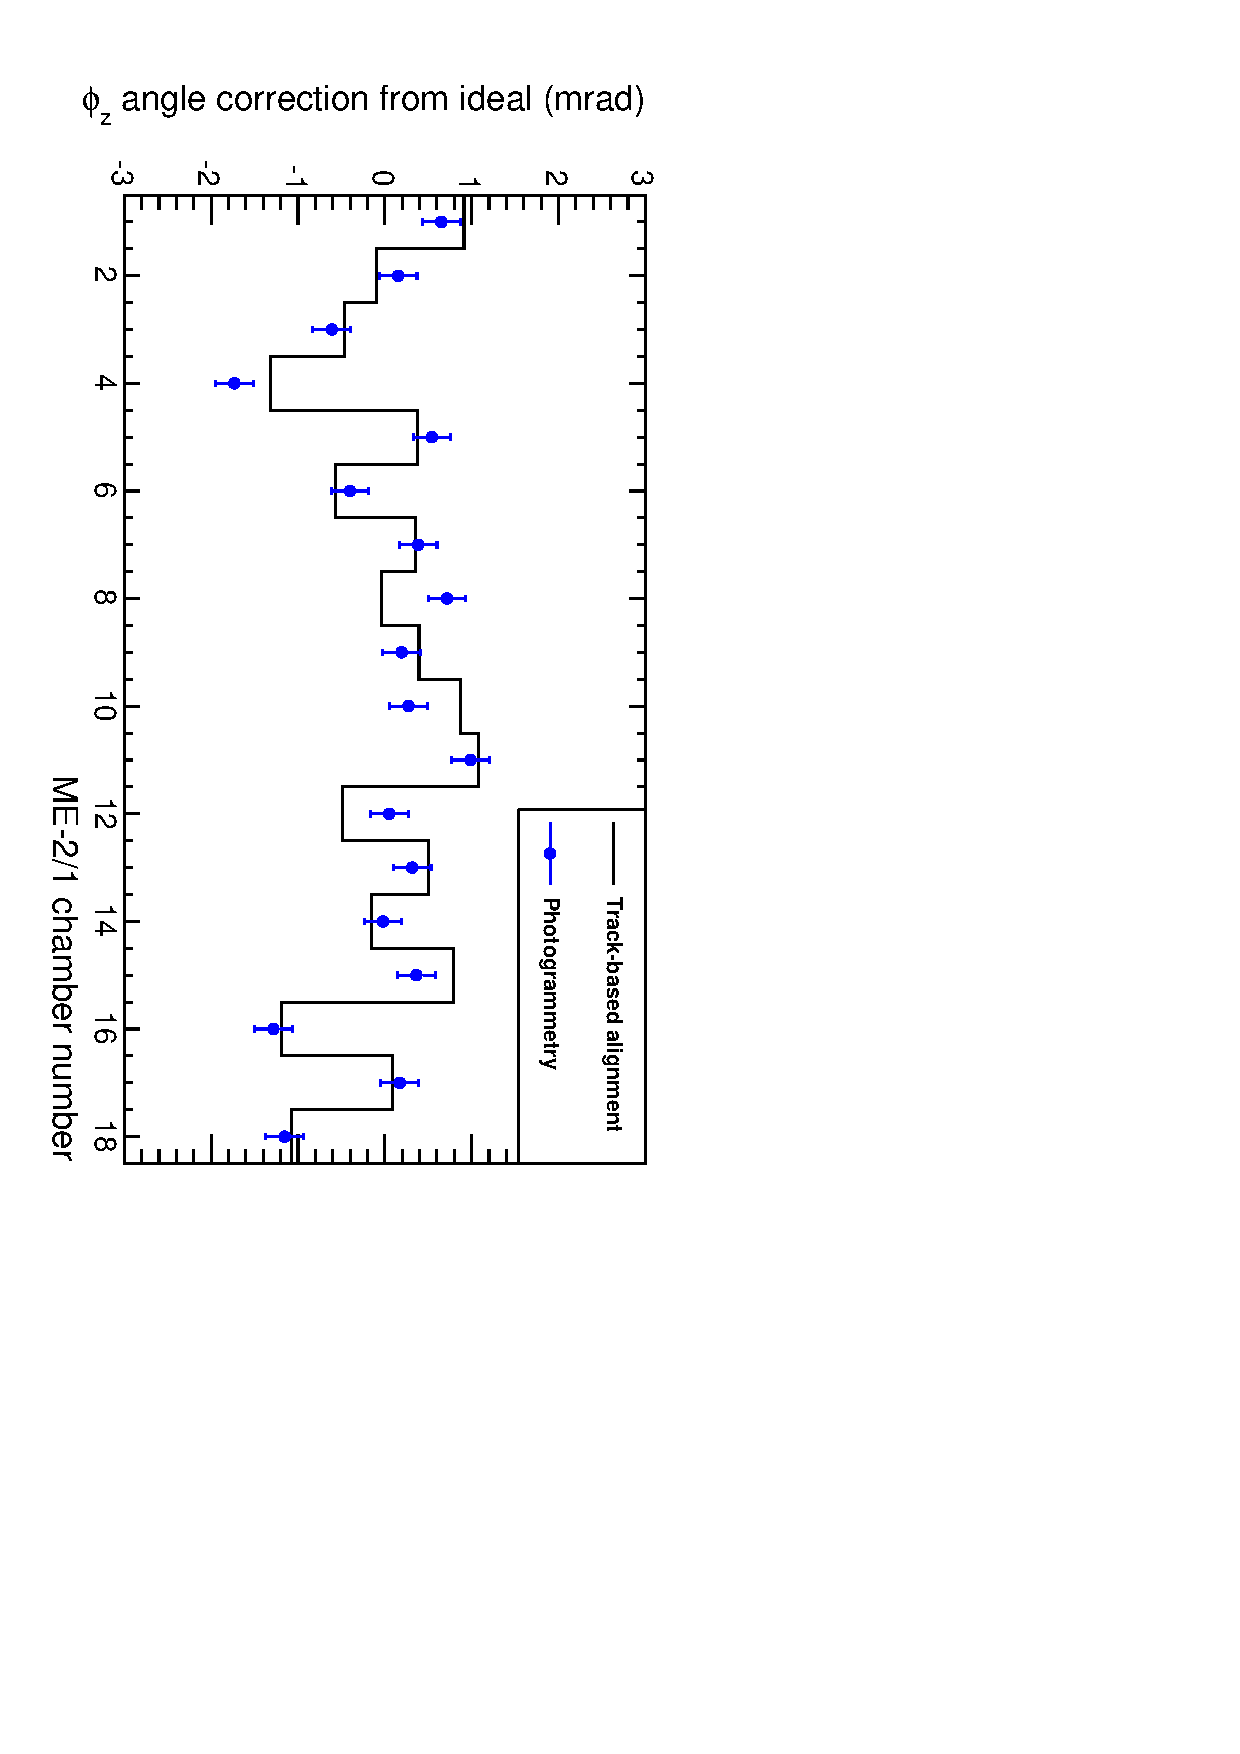
\includegraphics[height=0.95\linewidth, angle=90]{compare_m21_phiz.pdf}}\only<2>{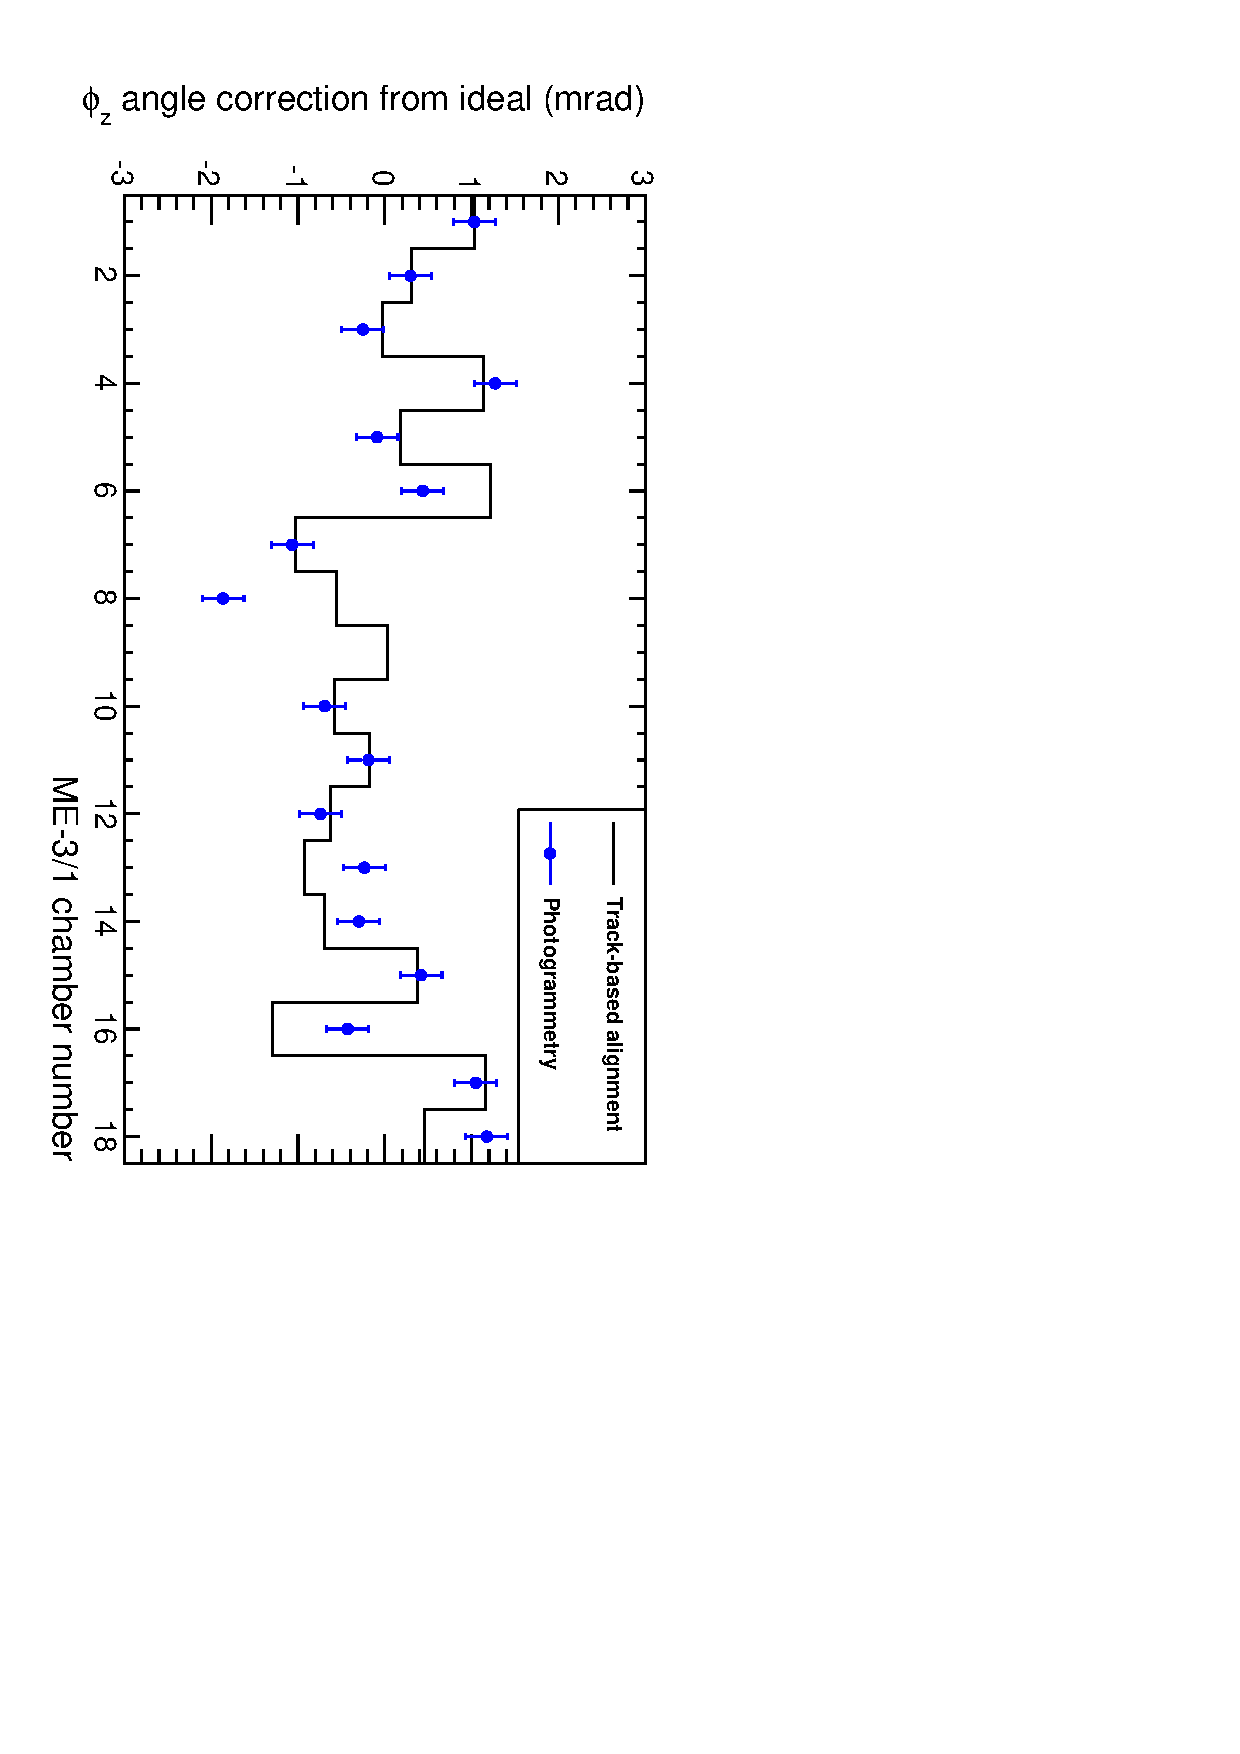
\includegraphics[height=0.95\linewidth, angle=90]{compare_m31_phiz.pdf}}
\end{columns}

%% \only<1>{\scriptsize Overlay of $r\phi$ translations, track-based and photogrammetry relative to ideal}
%% \only<2>{\scriptsize Overlay of $\varphi_z$ rotations, track-based and photogrammetry relative to ideal}
\end{frame}

\begin{frame}
\frametitle{Determine accuracy from PG}
\begin{itemize}
\item RMS difference between track-based and PG: 340~$\mu$m, 0.42~mrad
\item Photogrammetry $r\phi$ uncertainty is (300/$\sqrt{2}$)~$\mu$m = 210~$\mu$m
\item \textcolor{darkblue}{$r\phi$ errors in track-based method alone} = $\sqrt{340^2 - 210^2} =$ \textcolor{darkblue}{270~$\mu$m}
\item \textcolor{darkblue}{$\varphi_z$ errors} = $\sqrt{0.42^2 - (0.3\cdot\sqrt{2}\mbox{ mm}/1.85\mbox{ m})^2} =$ \textcolor{darkblue}{0.35~mrad}
\end{itemize}

\begin{columns}
\column{0.5\linewidth}
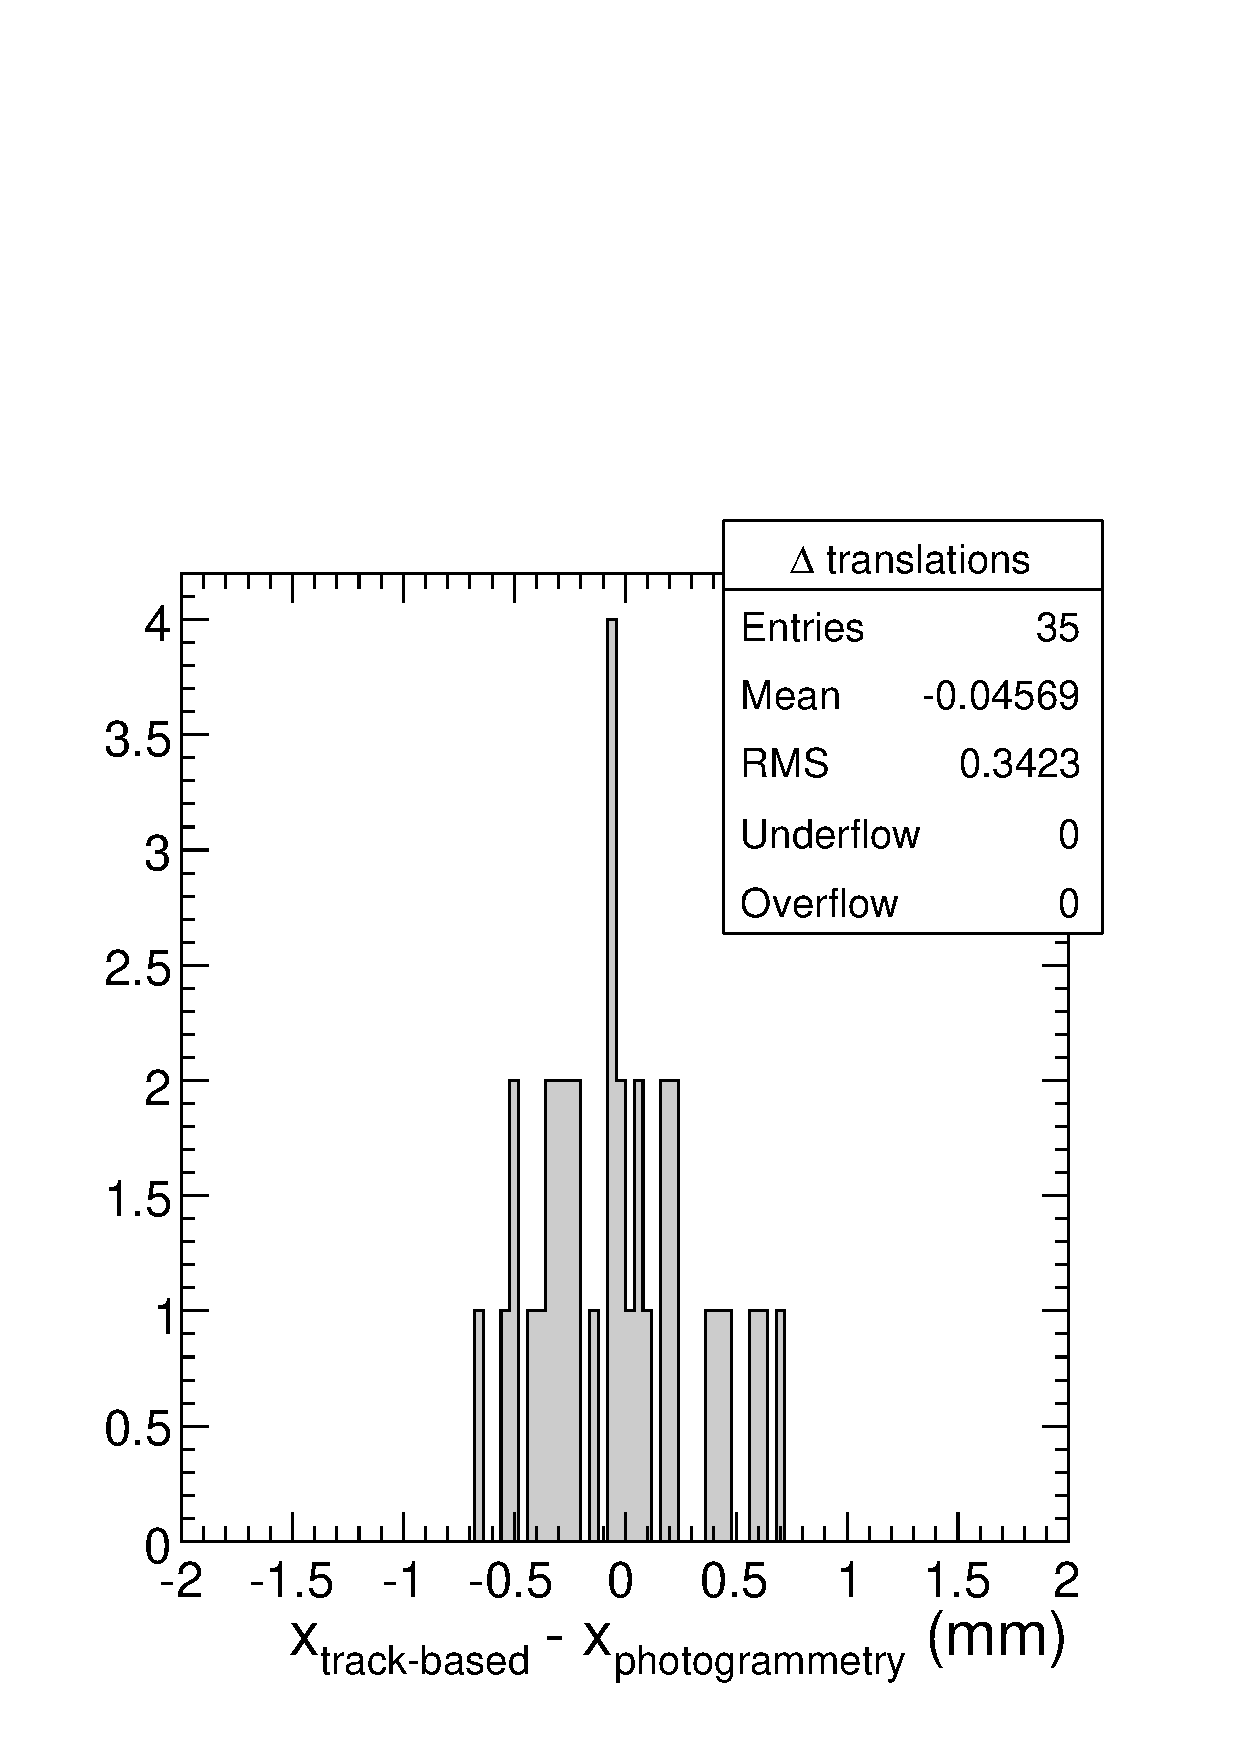
\includegraphics[width=\linewidth]{delta_translations.pdf}
\column{0.5\linewidth}
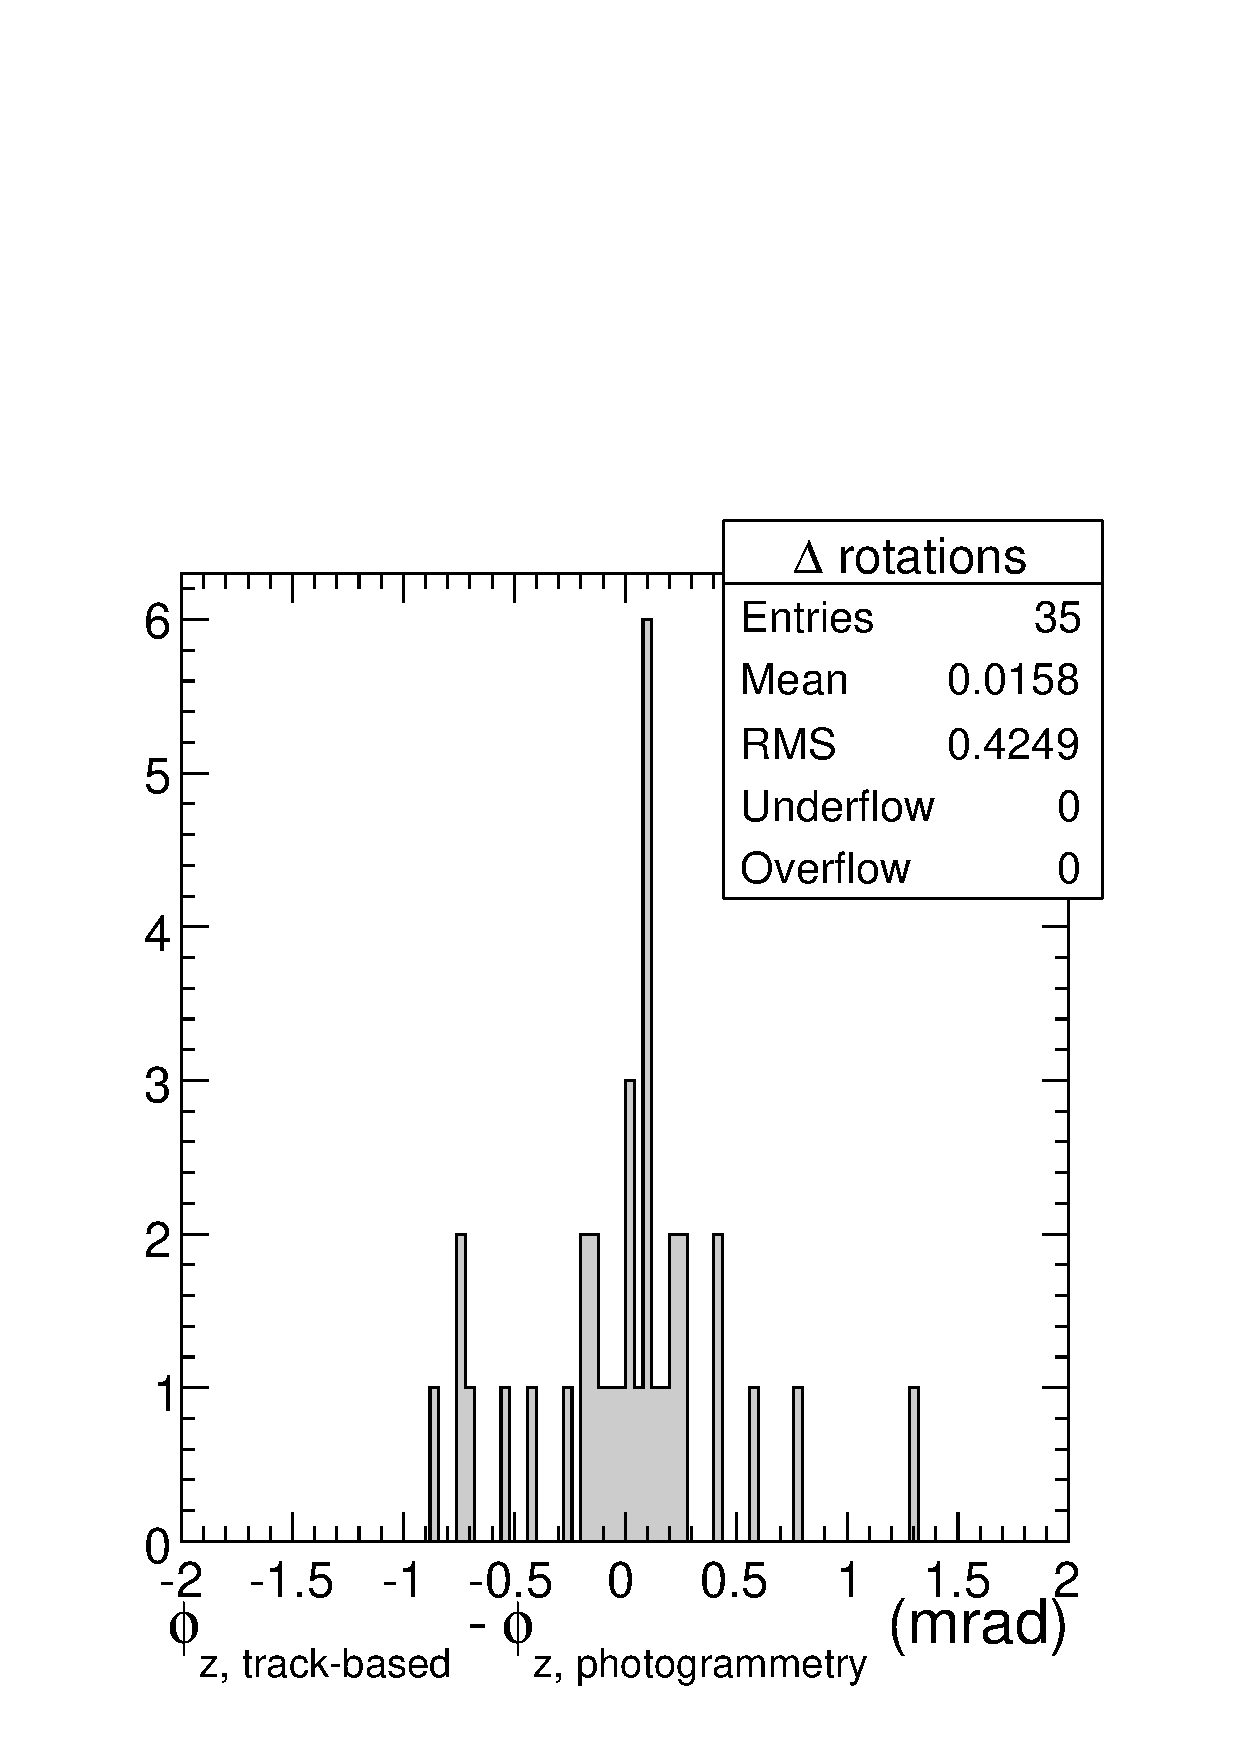
\includegraphics[width=\linewidth]{delta_rotations.pdf}
\end{columns}
\end{frame}

\begin{frame}
\frametitle{Ring consistency (closure)}
\begin{itemize}
\item Each residual distribution represents the difference in alignment between two chambers
\item Must sum to zero: $(x_1 - x_2) + (x_2 - x_3) + \ldots + (x_N - x_1) = 0$
\item $\varphi_y$ and $\varphi_z$ residuals have always summed to zero (``closed'')
\item $r\phi$ residuals closed in MC, but not in data
\item Agreement with photogrammetry ruled out possibility of alignment
  mistake; pointed to error in CMSSW chamber description
\begin{itemize}
\item active volume of chambers is 2.5~mm closer to beamline, {\it or}
\item active volume is 800~$\mu$m wider than in description
\end{itemize}
\item Oleg found 10~$\mu$m rounding error in strip width description
\begin{itemize}
\item multiplied by $\sim$80 strips $\approx$ 800~$\mu$m wider active volume
\end{itemize}
\item Implemented correction; ME$-$2/1, $-$3/1 closure is now perfect!

\begin{center}
\hspace{-1 cm} $\displaystyle \sum_{\mbox{\scriptsize chamber }i} (r\phi_i - r\phi_{i+1})$ \hspace{0.3 cm}
\begin{tabular}{c c c}
& before (mm) & after (mm) \\\hline
ME$-$2/1 & $+$14.30 & -0.72 $\pm$ 0.42 \\
ME$-$3/1 & $+$15.90 & -0.36 $\pm$ 0.51 \\
\end{tabular}
\end{center}

\end{itemize}
\end{frame}

\begin{frame}
\frametitle{Status of CSC Overlaps}
\begin{itemize}\setlength{\itemsep}{0.35 cm}
\item Strip geometry correction will go into CMSSW\_3\_0\_X \\ (where it
  won't introduce an error into the existing MC)
\item CSCOverlapsAlignmentAlgorithm will go into the new
  Alignment/MuonAlignmentAlgorithms directory for CMSSW\_3\_0\_X
\item Triggers and AlCa paths have been defined to collect overlaps
  data from beam-halo and collisions events
\begin{itemize}\setlength{\itemsep}{0.1 cm}
\item we'll probably keep using it into the collisions era, at least
  until globalMuon methods are fully validated
\item like the hardware system, it can provide quick monitoring \\ (in
  $r\phi$, $\varphi_z$, and to a lesser extent, $\varphi_y$)
\item not likely to work with a cosmic ray track source, but we only
  need something known to work with beam
\item these results are from 62232 (9 minutes of beam-2)
\end{itemize}
\end{itemize}
\end{frame}

%% \section*{First section}
%% \begin{frame}
%% \begin{center}
%% \Huge \textcolor{blue}{First section}
%% \end{center}
%% \end{frame}

\begin{frame}
\frametitle{CSC layer alignment}

\begin{itemize}
\item {\it First} first look at layer alignment by Karoly in MTCC
\item Internal chamber data can only simultaneously determine four
  layers and a straight track, insensitive to shear
\begin{itemize}
\item method of fixing track to layers 1 and 6:
\end{itemize}

\vspace{-0.5 cm}
\mbox{ } \hfill 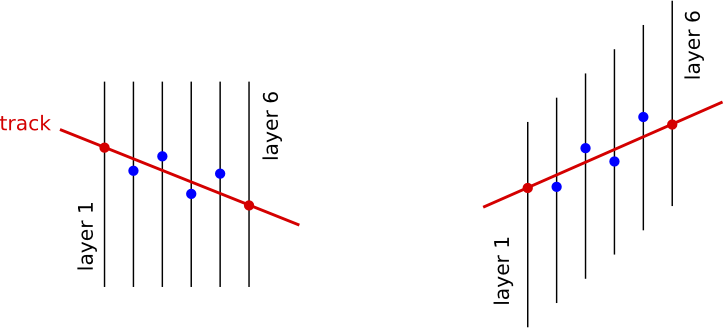
\includegraphics[width=0.65\linewidth]{layer_alignment_skew.png} \hfill \mbox{ }

\item Overlap events allow us to add one degree of freedom per chamber
\begin{itemize}
\item five layers is enough to describe complete internal alignment
\end{itemize}

\mbox{ } \hfill 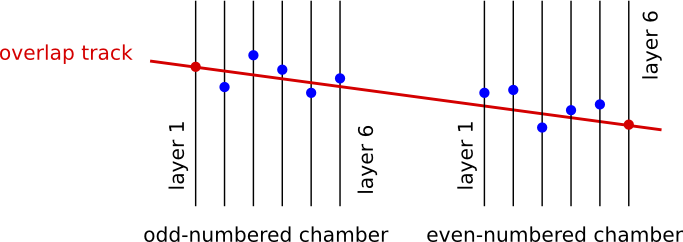
\includegraphics[width=0.65\linewidth]{layer_alignment_noskew.png} \hfill \hfill \hfill \mbox{ }

\end{itemize}
\end{frame}

\begin{frame}
\frametitle{Plots of layer residuals}

Test in \textcolor{darkblue}{Monte Carlo} with 36$\times$ statistics (folded all pairs)

\vspace{-0.15 cm}
\begin{itemize}
\item residuals (blue points) reproduce misalignment pattern (histogram)
\end{itemize}

\mbox{ } \hfill 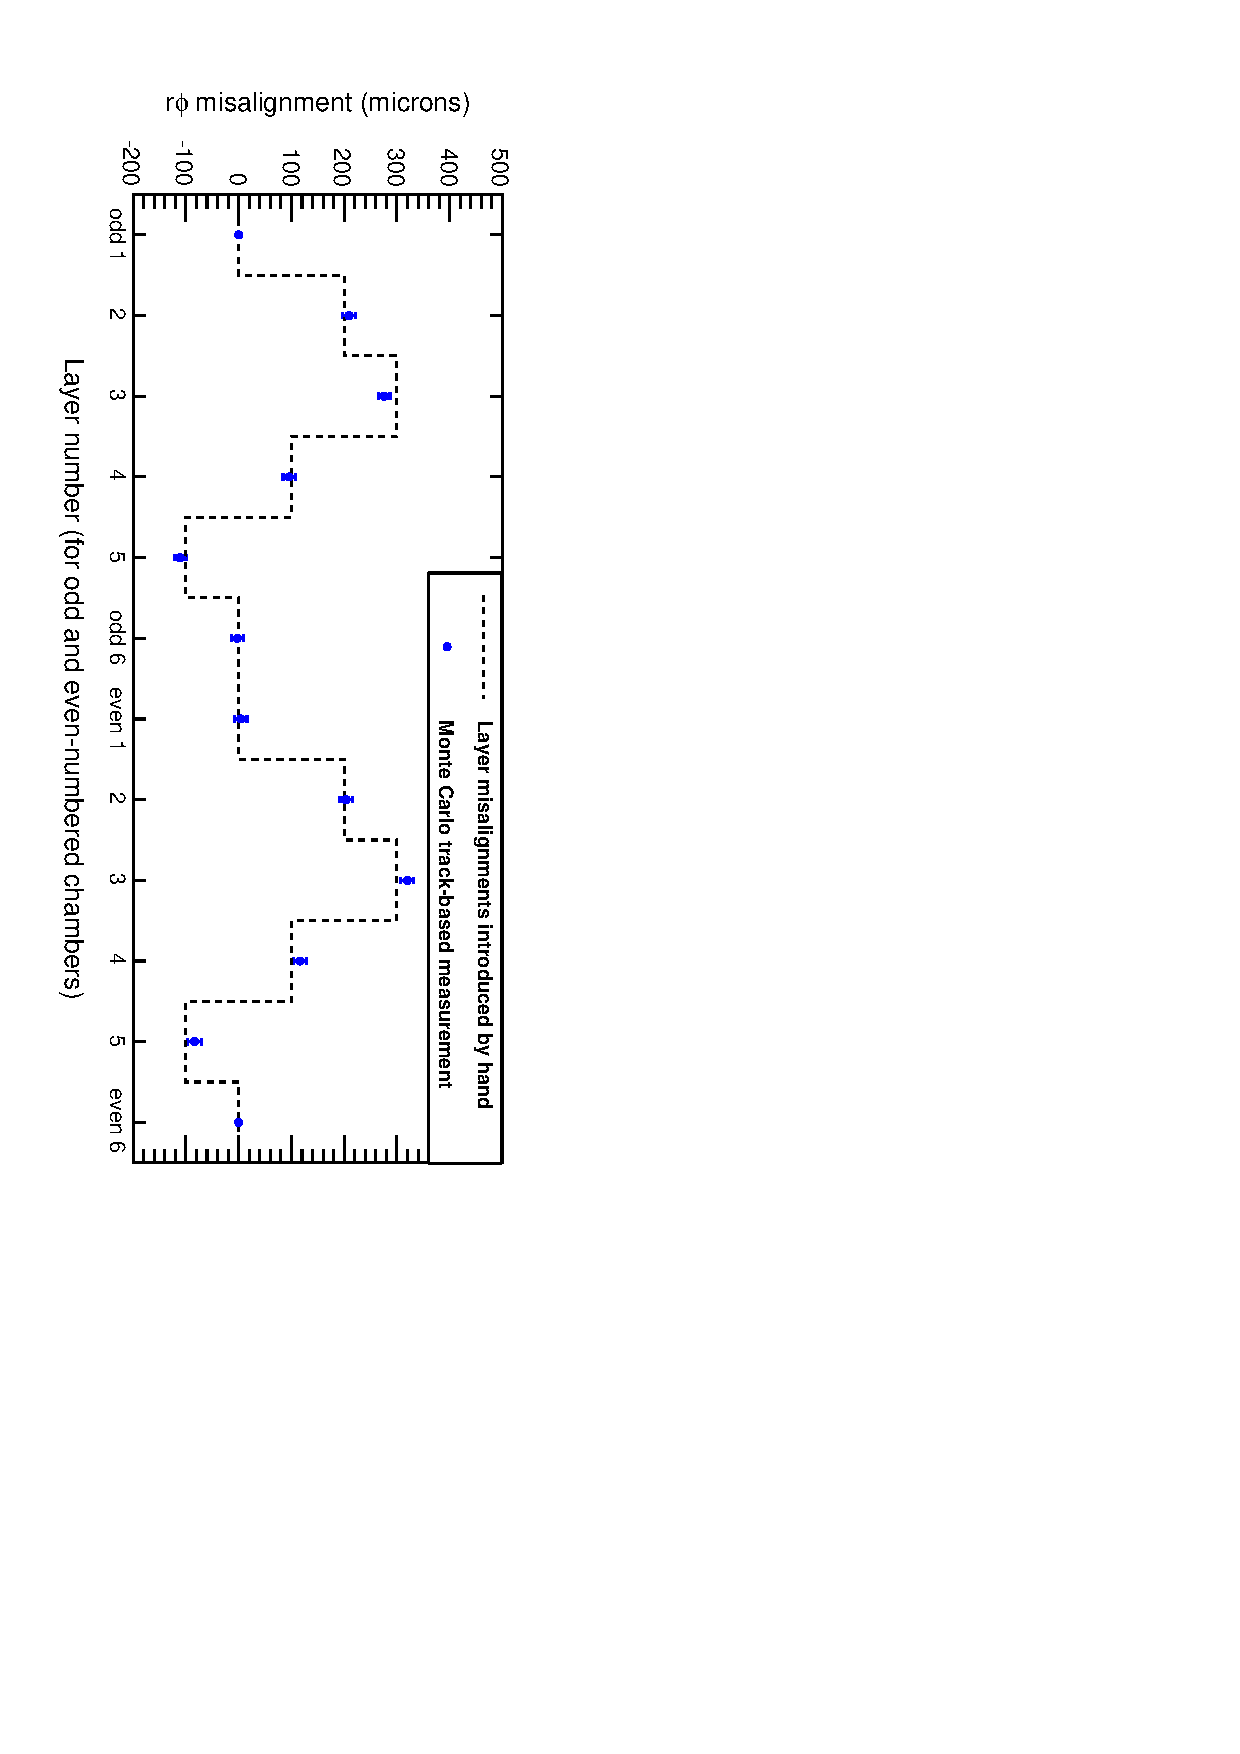
\includegraphics[height=0.8\linewidth, angle=90]{layer_test.pdf} \hfill \mbox{ }

Example in \textcolor{darkblue}{data}: chamber 7, layer 1 and chamber 8, layer 6 are fixed

\mbox{ } \hfill 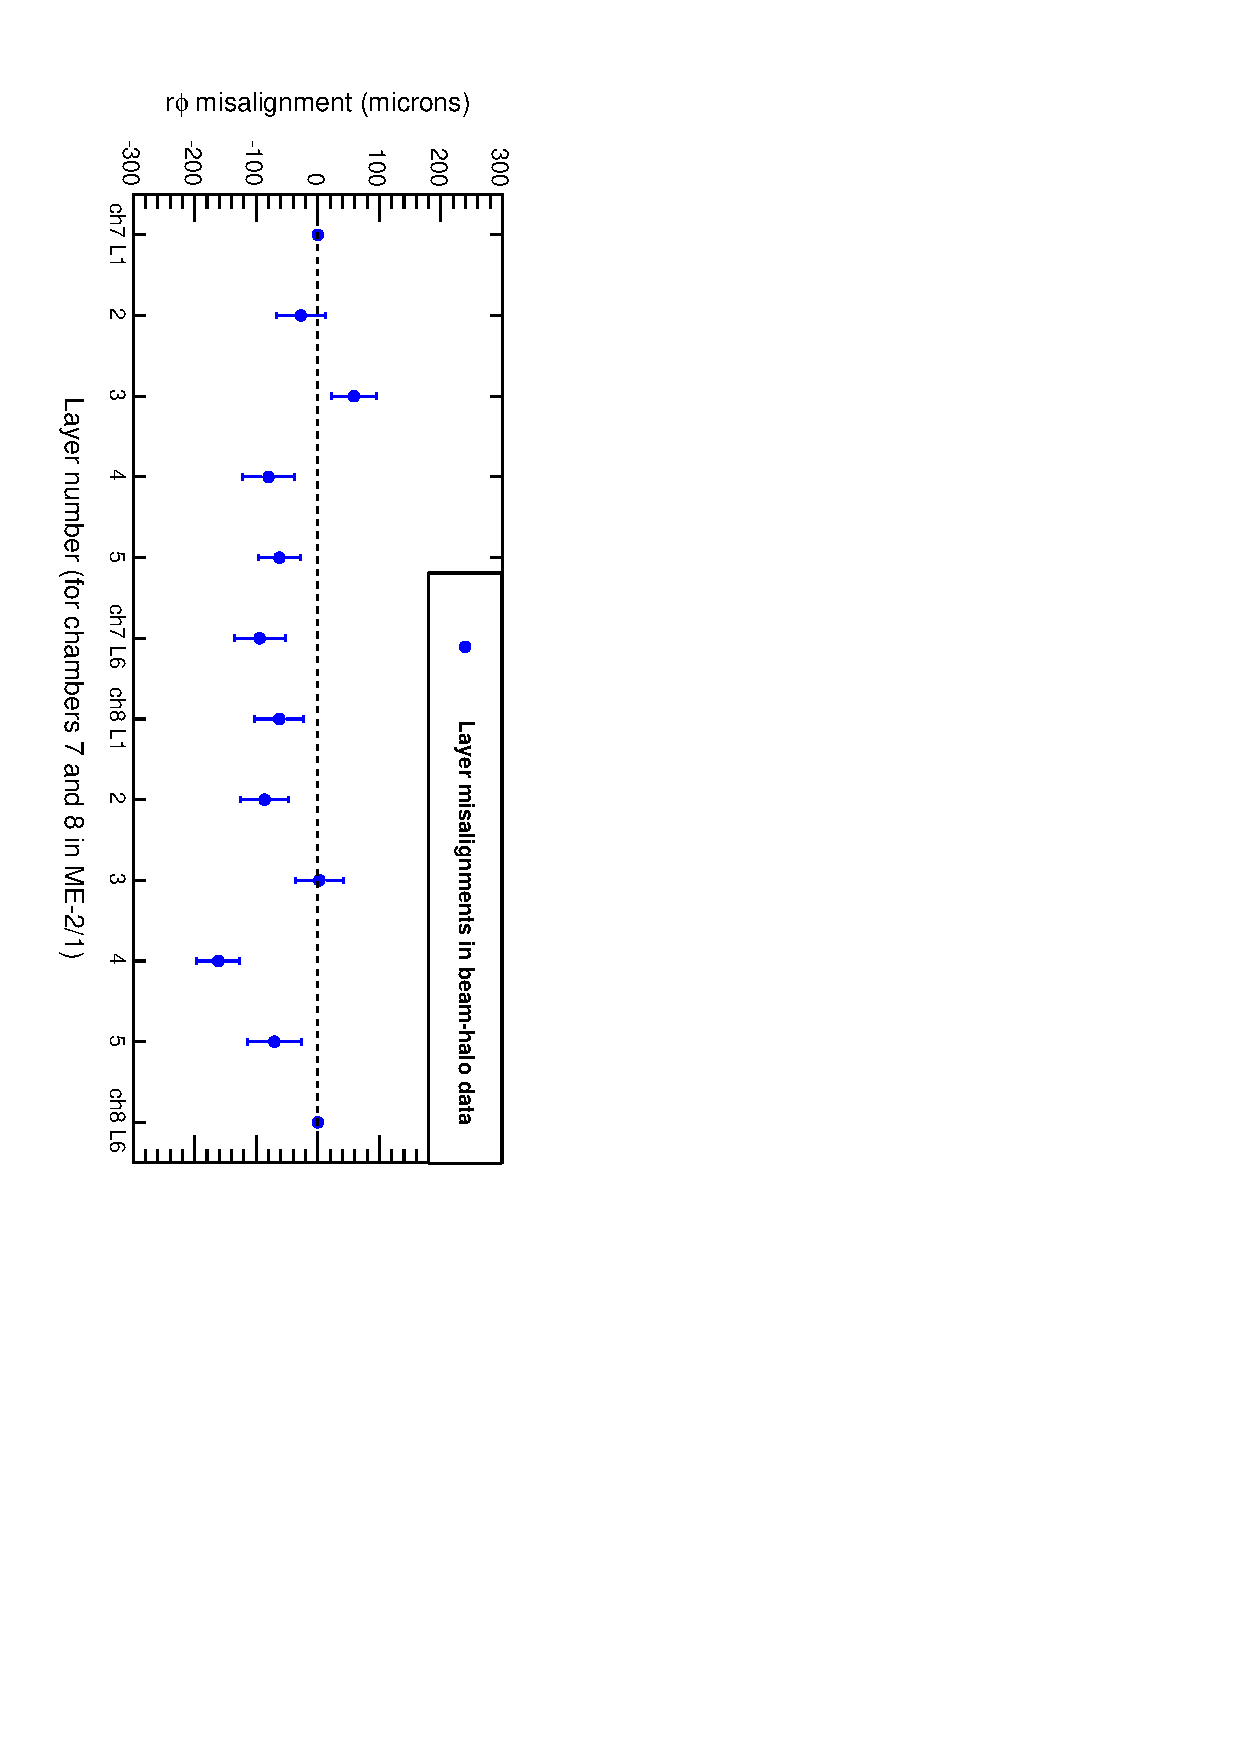
\includegraphics[height=0.8\linewidth, angle=90]{layer_data.pdf} \hfill \mbox{ }

\end{frame}

\begin{frame}
\frametitle{Typical scale and resolution}

\vspace{0.1 cm}
\begin{columns}
\column{0.6\linewidth}
\begin{itemize}
\item Observed $\sim$100~$\mu$m \mbox{layer misalignments\hspace{-0.25 cm}} in ME$-$2/1 and $-$3/1
\begin{itemize}
\item technique requires chambers to be previously aligned
\item (and must be followed by a chamber re-alignment)
\end{itemize}
\item About half as large as misalignments observed in MTCC
  \mbox{(which was ME$+$)\hspace{-1 cm}}
\item Resolution with full beam-halo run is 40--100~$\mu$m, hard to see misalignments
\end{itemize}

\column{0.4\linewidth}
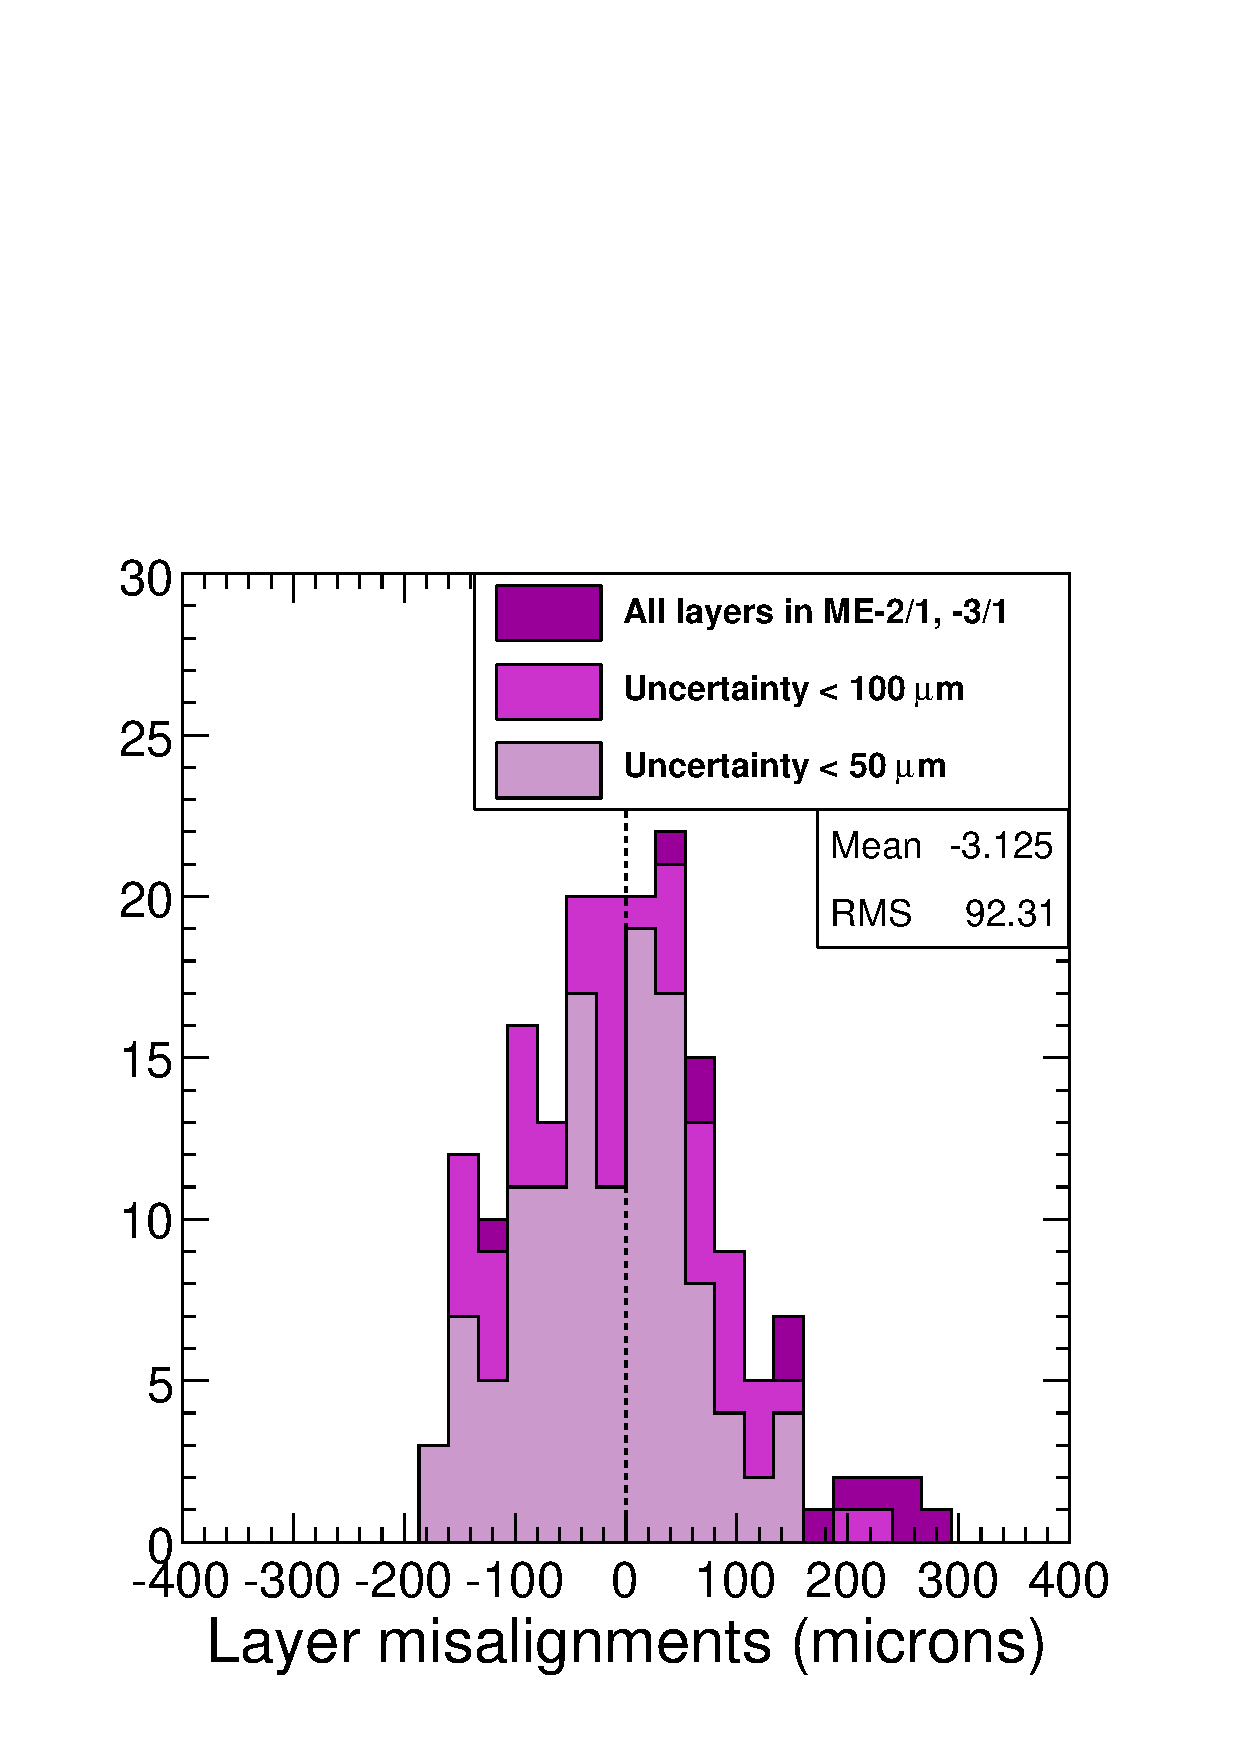
\includegraphics[width=\linewidth]{layer_hist.pdf}
\end{columns}

\vspace{0.1 cm}
\hspace{-0.45 cm} \begin{minipage}{0.9\linewidth}
\begin{itemize}
\item I have not cross-checked these with FAST measurements yet
\end{itemize}
\end{minipage}

\vspace{0.3 cm}
\hspace{-0.83 cm} \textcolor{darkblue}{\Large Status}

\begin{itemize}
\item Not yet integrated into an alignment routine: just illustrative plots
\item Layers only need to be aligned once
\item Definitive CSC layer alignment will probably be done with early \mbox{collisions\hspace{-1 cm}}
\end{itemize}
\end{frame}

\begin{frame}
\frametitle{Aligning endcap disks/rings}

\begin{itemize}
\item globalMuon statistics are very poor in the endcap, and the tight
  geometric cuts implied by the requirement that they pass through the
  tracker might be a source of bias

\item When we have a standAloneMuon refitter, this is what I have in mind for CRAFT:

\mbox{ } \hfill 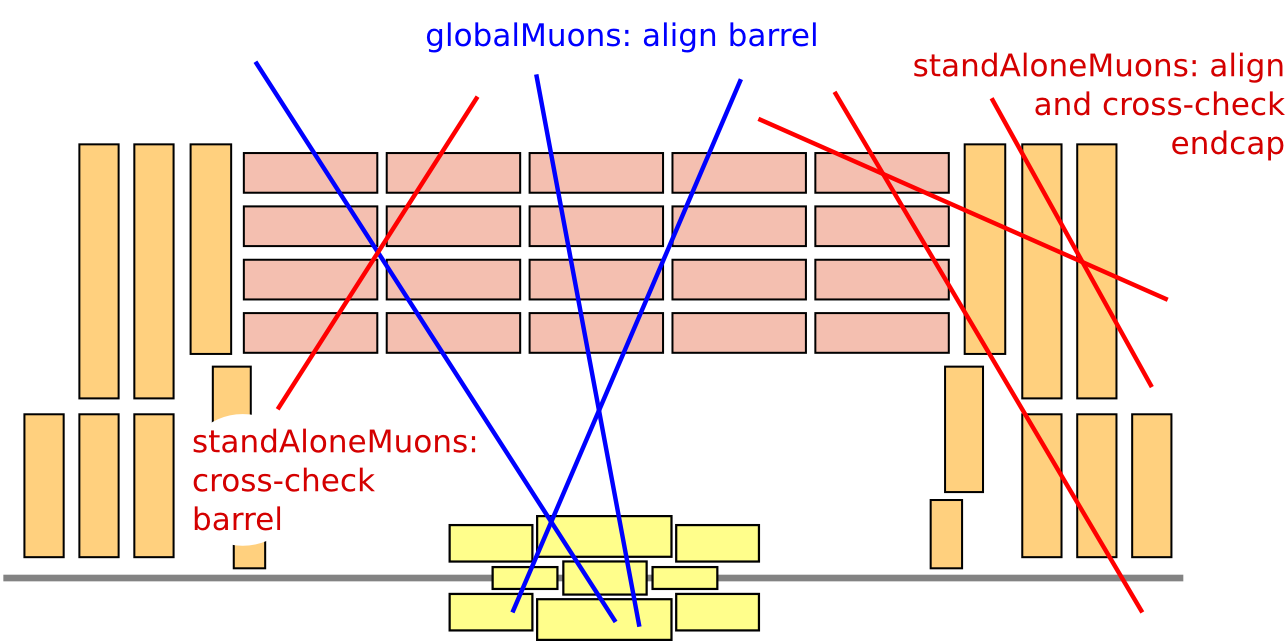
\includegraphics[width=0.9\linewidth]{globalMuons_and_standAloneMuons.png} \hfill \mbox{ }

\item These are the cross-checks that we did in CRUZET, with the addition of linking the barrel to the tracker
\end{itemize}
\end{frame}

\begin{frame}
\frametitle{Proposed combining procedure}

The following makes the best use of all available endcap data:

\vspace{0.2 cm}
\renewcommand{\arraystretch}{1.3}
\begin{tabular}{p{0.33\linewidth} p{0.4\linewidth} p{0.2\linewidth}}
Alignment step & Parameters updated & Responsible \\ \hline\hline
1.\ Photogrammetry & all but $\varphi_y$ for most chambers & Karoly \& Oleg \\ \hline
2.\ Straight-line monitors & $r\phi$, $z$, $\varphi_x$, $\varphi_z$ for monitored chambers, averages for the rest & Florida Tech \\ \hline
3.\ CSC Overlaps & $r\phi$, $\varphi_y$, $\varphi_z$ for all chambers, keeping average of monitored chambers fixed & Texas A\&M \\ \hline
4.\ Disk alignment & whole-disk 6 d.o.f.\ & Texas A\&M \\ \hline\hline
\end{tabular}

\vfill
\begin{itemize}
\item In the end, photogrammetry supplied the radial positions, SLMs
  provide $z$ and $\phi_x$ of disk-bulging and the $r\phi$ connection
  between rings, Overlaps provide $r\phi$, $\varphi_y$, and
  $\varphi_z$ of individual chambers, and Disk alignment connects to
  the tracker (or barrel if there are still globalMuon issues)
\item Communication at each step proceeds through CSCAlignmentRcds
\end{itemize}
\end{frame}

\begin{frame}
\frametitle{Conclusions}
\begin{itemize}\setlength{\itemsep}{0.75 cm}
\item CSC Overlaps procedure is in good shape

\item CSC layer alignment can be done with many of the same tools

\item StandAlone refitter for cosmics will allow us to do deeper
  cross-checks of globalMuons and align the endcap disks

\item Proposed a procedure for combining results from our
  complimentary alignments
\end{itemize}

\vfill
\mbox{ }
\label{numpages}
\end{frame}

\end{document}
